\documentclass[twoside,nogutter]{glasgowthesis}
%\documentclass[twoside,hidelinks]{glasgowthesis}
% ^^ draft shows overfilled boxes (but disables links)
% ^^ replace "oneside" with "twoside" to set the gutter correctly for
%    two-sided printing.
% ^^ add "nogutter" option for digital copy (without binding offsets),
%    if printed copy is twoside, use [twoside,nogutter] for digital copy.
% ^^ add "hidelinks" option to remove coloured links (e.g. for printing)

%%%
% Packages

\usepackage{graphicx}
\usepackage{amsmath}
\usepackage{amssymb}
\usepackage{color}
\usepackage{bookmark}
\usepackage{hyphenat} % for \hyp{} instead of "-".

%%%
% Bibliography

% import package and set some options
\usepackage[minnames=1,maxnames=5,style=numeric-comp,sorting=none,backend=bibtex]{biblatex}

% set path to database
\bibliography{bibliography.bib}

%%%
% SI units

% import package, with astronomy units
\usepackage[separate-uncertainty=true,alsoload=astro]{siunitx}

% for nice display of negative symbol in equations
\sisetup{
   detect-mode,
   detect-family,
   detect-inline-family=math,
}

% sqrt(Hz)
\DeclareSIUnit{\sqrthz}{\ensuremath{\sqrt{\textrm{\hertz}}}}

%%%
% List of symbols, definitions, etc.

% import package
\usepackage[acronym,nomain]{glossaries}

% make the list
\makeglossaries

%%%
% superscript th, st, nd, rd, etc.
\usepackage[super]{nth}

%%%
% Hyperlinks
%
% (This should be as close to the end of the package imports as possible - see https://www.tug.org/applications/hyperref/manual.html)

% import package
\usepackage{hyperref}
\hypersetup{
  colorlinks=true,
  linkcolor=blue,
  filecolor=magenta,      
  urlcolor=cyan
}

%%%
% Fix silly LaTeX space/punctuation behaviour with custom commands
%
% The command '\xspace' should be added to the end of custom commands which lack arguments, to make LaTeX put a space after the command's output.
\usepackage{xspace}

%%%
% Smaller text in captions
\usepackage[font=small]{caption}

%%%
% Subcaptions
\usepackage{subcaption}

%%%
% Wrapping text around figures and tables
\usepackage{wrapfig}

%%%
% Formatting of ordinal numbers, i.e. 1st, 2nd, 3rd, as superscripts
\usepackage[super]{nth}

%%%
% Chemical symbols
\usepackage[version=3]{mhchem}

%%%
% Code listings
% https://www.ctan.org/tex-archive/macros/latex/contrib/listings/
\usepackage{listings}

%%%
% Custom commands

% command to make plural versions of commands (http://tex.stackexchange.com/questions/259287/how-to-define-a-newcommand-that-expands-into-another-newcommand)
% e.g.
% 	\makename[es]{veggie}{potato}
% makes the commands \veggie (=potato) and \veggies (=potatoes)
\newcommand{\makename}[3][s]{%
  \expandafter\newcommand\csname #2\endcsname{#3\xspace}%
  \expandafter\newcommand\csname #2s\endcsname{#3#1\xspace}%
}

% red, italic, bold - for notes
\newcommand{\note}[1]{\textcolor{red}{\emph{[\textbf{Note: }#1]}}}

% blue, normal text - for statements that need fact-checked
\newcommand{\checkme}[1]{\textcolor{blue}{#1}}

% naive with diaeresis
\newcommand{\naive}{na\"ive\xspace}

% et al.
% (and a backslash to prevent TeX thinking a new sentence starts afterwards)
\newcommand{\etal}{et~al.\@}

% gravitational wave detectors
\newcommand{\GEO}{GEO 600}
\newcommand{\GEOHF}{GEO \gls{HF}}
\newcommand{\LIGO}{\gls{LIGO}}
\newcommand{\LLO}{\LIGO{} Livingston}
\newcommand{\LHO}{\LIGO{} Hanford}
\newcommand{\ILIGO}{Initial \LIGO{}}
\newcommand{\ALIGO}{Advanced \LIGO{}}
\newcommand{\INDIGO}{\gls{LIGO} India}
\newcommand{\LIGOCE}{\gls{LIGO} Cosmic Explorer}
\newcommand{\VIRGO}{Virgo}
\newcommand{\AVIRGO}{Advanced \VIRGO{}}
\newcommand{\KAGRA}{\gls{KAGRA}}
\newcommand{\ET}{Einstein Telescope}
\newcommand{\ETLF}{\gls{ET}-\gls{LF}}
\newcommand{\ETHF}{\gls{ET}-\gls{HF}}

% Michelson interferometer
\newcommand{\MI}{Michelson interferometer\xspace}

% Fabry-Perot with accent
\newcommand{\FP}{Fabry-P\'{e}rot\xspace}

% Fabry-Perot Michelson interferometer
\newcommand{\FPMI}{\FP{} \MI{}\xspace}

% Dual-recycled Fabry-Perot Michelson interferometer
\newcommand{\DRFPMI}{Dual-recycled \FPMI{}\xspace}

% speedmeter
\newcommand{\SM}{speedmeter\xspace}

% Sagnac Speedmeter
\newcommand{\SSM}{Sagnac \SM{}\xspace}

% Sagnac Speedmeter experiment
\newcommand{\SSMEXPT}{\SSM{} experiment\xspace}

% AEI 10m prototype
\newcommand{\AEIPROTOTYPE}{AEI \SI{10}{\meter} prototype\xspace}

% Glasgow 10m prototype
\newcommand{\GLASGOWTENM}{Glasgow \SI{10}{\meter} prototype\xspace}

% LIGO Scientific Collaboration
\newcommand{\LSC}{\gls{LIGO} Scientific Collaboration\xspace}

% Matlab
\newcommand{\MATLAB}{Matlab\xspace}

% L minus
\newcommand{\LMINUS}{$L_{\left(-\right)}$}

% L plus
\newcommand{\LPLUS}{$L_{\left(+\right)}$}

% Scultety
\newcommand{\SCULTETY}{Scult\'{e}ty}

% title, contents, etc.
\frontmatter
%%%
% Document

\begin{document}

%\pagestyle{empty}
%\pagenumbering{gobble}

\title{Enhancing the Sensitivity of Future Laser-Interferometric Gravitational Wave Detectors}
\author{Sean Stephan Leavey}
\date{Month Year}

\maketitle

\cleardoublepage

\input{"00-abstract.tex"}
%\addcontentsline{toc}{chapter}{Abstract}

\newpage
\input{"00-acknowledgements.tex"}
%\addcontentsline{toc}{chapter}{Acknowledgments}

\cleardoublepage
\vspace*{1.75in}
\begin{flushright} Dedication. (Is what you need.)\end{flushright}


%\pagenumbering{roman}
%\setcounter{page}{1}

% -----------------------------------------------------------------------------
\newpage

\vspace*{1.75in}
\begin{center} {\bf Creative Commons Licence}\end{center}
\noindent I hereby grant permission under the following terms...

\begin{description}
\item Sean Stephan Leavey\ \\ \ \\ \ \\
\hrule
\end{description}
\newpage

% -----------------------------------------------------------------------------

% import glossary terms
\input{"00-definitions.tex"} 

% -----------------------------------------------------------------------------
\newpage
%\thispagestyle{empty}

\addcontentsline{toc}{chapter}{Preliminaries}

% change contents title to lower case
\renewcommand{\contentsname}{Table of contents}
\tableofcontents

\listoftables
\addcontentsline{toc}{section}{List of tables}

\listoffigures
\addcontentsline{toc}{section}{List of figures}

\printglossaries
\addcontentsline{toc}{section}{List of acronyms and symbols}

% -----------------------------------------------------------------------------
\cleardoublepage

% Number chapter boomarks
\bookmarksetup{numbered}

\section*{\label{c:intro:thesisstatement}Thesis statement}
\addcontentsline{toc}{section}{Thesis statement}

\input{"00-statement.tex"}

\newpage

\section*{\label{c:intro:credits}Credits}
\addcontentsline{toc}{section}{Credits}

\input{"00-credits.tex"}

% main chapters
\mainmatter
\chapter{\label{c:gw-detection}Gravitational waves}

\section{Event GW150914}
Around \num{1.3} billion years ago a pair of black holes, one with \num{36} solar masses and the other with \num{29} solar masses, merged into a single black hole with \num{62} solar masses \cite{Abbott2016}. The missing energy equivalent to \num{3} solar masses was radiated away in the form of gravitational waves.

At 09:50:45 \gls{UTC} on \nth{14} September 2015, gravitational waves from the event reached the \LIGO{} Livingston detector, perturbing the mirrors by \SI{e-18}{\meter} and creating a signal large enough for the electronics controlling the interferometer to detect the ripple in spacetime more than \num{23} times above the background noise. Seven milliseconds later, the same wavefront passed the \LIGO{} Hanford detector and moved the mirrors in the opposite direction. Meanwhile, computerised data analysis pipelines searching for coincident signals in each detector were running, and identified the event within a few minutes. Subsequent offline analysis using template banks representing waveforms produced by sources with different parameters were matched to the signal to calculate the most probable values. Given the significance of the signal above the detector's noise, and its fit to the templates, it was clear that the first detection of gravitational waves had been made.

The waveforms for event \emph{\GWFIRSTEVENT{}}, as it has become known, are consistent with a binary black hole merger in that they were swept up in frequency before creating a loud ``chirp'' signal as shown in Figure\,\ref{fig:gw150914}. The signal was only above each detector's background noise for the last few \SI{}{\milli\second} of this process, but it was consistent enough with theory that the collaboration could report a false alarm rate of less than \num{1} in \num{200000}. Not only did \LIGO{} make the first observation of a gravitational wave, it also made the first detection of a binary black hole system and found the missing experimental proof of Einstein's theory of general relativity. The field opening up due to \LIGO{} and the worldwide network of detectors in operation and under assembly, \GEO{}, \VIRGO{} and \KAGRA{}, represents an opportunity to study the universe in a completely new way.

\begin{figure}
  \centering
  \includegraphics[width=\columnwidth]{graphics/generated/from-python/10-gw150914.pdf}
  \caption[Measured strain from the LIGO Hanford and Livingston detectors around the time of event \GWFIRSTEVENT{}]{\label{fig:gw150914}Measured strain from the \LIGO{} Hanford and Livingston detectors around the time of event \GWFIRSTEVENT{}. Fast data pipelines work to find the best fitting template for the calibrated detector measurements from precomputed banks representing the various combinations of the system's parameters. Beyond this initial identification, computationally intensive analysis of the data around the time of the candidate event is processed using a variety of techniques to identify the most likely source parameters, and these can later be matched to numerical relativity models. The numerical relativity models best fitting the analysed data are shown for each site in the lower panel. These curves were originally presented in \cite{Abbott2016}, and they have been passed through a \num{35} to \SI{350}{\hertz} bandpass filter to remove higher and lower frequency background noise unrelated to the signals.}
\end{figure}
% data from https://losc.ligo.org/events/GW150914/
% Low frequency noise on the numerical relativity waveform is from the fact that the noise floor PSD of the detector is noisier than at high frequencies. This is probably because there is less data to FFT at lower frequencies by definition. So essentially it comes from the fact that the data was whitened first.

\section{Scientific outcomes from the first joint observation run}
The first detection was made shortly before a science run in which the two \LIGO{} detectors were kept at their most sensitive operating conditions as often as possible for a period of three months. In that time a second detection was made of a separate binary black hole merger, \GWSECONDEVENT{} \cite{Abbott2016b}, and taken alongside the first detection and another signal with lower significance it was possible for the \LSC{} and \VIRGO{} collaboration to make some important scientific discoveries. Among the outcomes from the observation run were that the first experimental tests of strong gravitational fields present during the events were still consistent with general relativity \cite{Abbott2016c}; that ``heavy'' black holes exist in nature and that they probably formed in an environment with low metallicity \cite{Abbott2016d}; and that the rate at which binary black holes merge in the known universe is constrained given the observations to between 9 and 240 per cubic gigaparsec per year \cite{lscvirgoo1}, suggesting that the advanced detectors might see dozens more in subsequent science runs.

Beyond the detection of binary black hole mergers, other sources such as compact neutron star binaries have yet to be found but are predicted to exist producing signals within the sensitivity of the detector networks for future science runs \cite{Abbott2016f}. Subsequent observations will hope to probe for new sources of gravitational waves, and with longer integration time it will be possible to set improved limits on the population of some of these astrophysical objects in our universe.

The long term goal of researchers in the field is to assemble a worldwide network of gravitational wave detectors to compliment the existing network of electromagnetic (\gls{EM}) telescopes to facilitate \emph{multi-messenger} astronomy. Such a network would be able to localise the sky position incident gravitational waves well enough to allow for \emph{\gls{EM} follow-up} \cite{Abbott2016e, Abbott2016f}, whereby the data from both telescopes and gravitational wave detectors can be combined to probe the astrophysics of the events in unprecedented detail and to identify and learn more about the nature and origin of host galaxies.

\section{General relativity and gravitational waves}
A consequence of Einstein's theory of general relativity, gravitational waves are produced by changes in the quadrupole moment of mass distributions such as the presence of non-spherical asymmetries in spinning objects or pairs of objects coalescing with elliptical orbits. The effect a gravitational wave has on spacetime as it propagates is to stretch it in one direction whilst contracting it in another. This \emph{strain} can be expressed as a linear combination of ``plus'' and ``cross'' polarisation terms, shown for an initially circular ring of test particles on a 2D plane as a function of phase angle in Figure\,\ref{fig:gravitational-wave-polarisation}.

\begin{figure}
  \centering
  \includegraphics[width=\columnwidth]{graphics/generated/from-svg/10-gravitational-wave-polarisation.pdf}
  \caption[Plus and cross polarisations of a propagating gravitational wave]{\label{fig:gravitational-wave-polarisation}Plus and cross polarisations of a propagating gravitational wave. As the wave travels, shown in this depiction perpendicularly to the plane of this page, it stretches spacetime in one direction while contracting it in the other in an elliptic behaviour. A gravitational wave can be described as a linear combination of the two polarisations.}
\end{figure}

Although in principle gravitational waves can be produced by all massive bodies, gravitational waves from Earth-bound objects, including the Earth itself, are not even remotely detectable. The strain in spacetime produced by such objects is so weak that there is no hope for us to make such a detection with any known technology. A good estimate for the strain produced by a pair of rotating objects is given as \cite{Sathyaprakash2009}:
\begin{equation}
  \label{eq:happrox}
  h \lesssim \frac{2 G \left( M v^{2} \right)_{\text{nonspherical}}}{c^4 r},
\end{equation}
where $G$ is the gravitational constant, $\left( M v^{2} \right)_{\text{nonspherical}}$ is the kinetic energy associated with the non-spherical parts of the source required for the creation of gravitational waves, $c$ is the speed of light and $r$ is the distance between the source and the detector. To get an idea of what the strain would be for man-made sources, we can consider as in \cite{Sathyaprakash2009} the case of two cars of mass $M = \SI{e3}{\kilo\gram}$ attached to opposite ends of a rod of length $d = \SI{10}{\meter}$, spinning about its centre in a centrifuge at a frequency of $f = \SI{10}{\hertz}$. The tangential velocity of the cars will be around $2 \pi f d \approx \SI{600}{\meter\per\second}$, about as fast as a modern fighter jet. Placing the detector one wavelength away, and using Equation\,\ref{eq:happrox}, the strain turns out to be around $\SI{4e-43}{}$. To be able to detect such a strain the current most sensitive detectors, \ALIGO{}, would require an improvement in sensitivity of \SI{20}{} orders of magnitude, which is clearly ludicrous.

A pair of solar-mass objects orbiting each other at \SI{100}{\hertz} within \SI{50}{\mega\lightyear} produces a strain of only one part in \SI{e21}{}, which is an amount only now detectable after decades of detector development. It is only the waves produced by the most violent redistribution of matter in the heaviest, most compact systems in the universe which we have any chance of detecting: binary black holes, compact binary neutron stars and core-collapse supernovae amongst others. Even then, gravitational radiation is only produced by the presence of a changing quadrupole moment and so only a subset of sources that happen to be in coalescence or contain surface asymmetries produce waves we have the ability to detect.

\section{Development of the gravitational wave detector}
Using the \emph{local Lorenz} gauge an incident gravitational wave can be described as a change in the distance separating two reference points in spacetime, and so a measurement of the length between pairs of test masses placed at the different points on the edges of the ellipses shown in Figure\,\ref{fig:gravitational-wave-polarisation} can be made to infer the presence of passing gravitational waves. Given the behaviour of the propagating waves, the primary degree of freedom they excite in such an apparatus is the differential mode of the distance separating the test masses, \LMINUS{}, which can be defined in terms of the position of the test masses $x_{\text{A}}$ and $x_{\text{B}}$ as:
\begin{equation}
  \label{eq:darm}
  \textrm{\LMINUS{}} = \frac{x_{\text{A}} - x_{\text{B}}}{2}.
\end{equation}
The strain of an incident gravitational wave, $h_0$, can be determined from the measured differential change in length between the test masses given the distance nominally separating the test masses, $L$:
\begin{equation}
  \label{eq:gw-strain}
  h_0 = \frac{\text{\LMINUS{}}}{L}.
\end{equation}

\subsection{Resonant bars}
The first attempts to detect gravitational waves began with Joseph Weber's studies in the 1960s with his \emph{Weber bar} \cite{Weber1960}. This was a device developed to act as a direct strain meter, with incident gravitational waves exciting the separation of the material along the length of the bar. Piezoelectric sensors placed on the surface of an aluminium cylinder convert changes in length into electrical signals. Whilst the expected change in length of such a cylinder from gravitational radiation would in most cases be tiny, the resonant frequency of the cylinder, typically in the kilohertz range, acts to enhance the amplitude of the length change at nearby frequencies. The sensitivity of such a bar as a function of frequency is determined in part by its quality factor (Q), with a necessary trade-off being made between peak sensitivity (high Q) and detection bandwidth (low Q). As sources of gravitational radiation are almost universally weak, the only reasonable hope of making such a detection is to choose a high Q material and hope for a favourable signal frequency.

Despite improvements over the following decades, the peak sensitivity of state-of-the-art resonant bar detectors was surpassed by \emph{interferometric} gravitational wave detectors in 2003 \cite{Pitkin2011} after it was shown that \emph{second generation} detectors improving upon the initial designs would offer superior sensitivity across a much wider bandwidth \cite{Harry2002a}. The interferometer was first suggested as a means for gravitational wave detection shortly after the introduction of the Weber bar \cite{Pustovoit1962}, but efforts to build prototypes and understand the significant sources of noise only gained momentum in the 1970s \cite{Moss1971, Weiss1972}.
% Gertsenshtein and Pustovoit contains: "We shall show below that this corresponds to a secondary effect, namely to resonant excitation of gravitational waves by the electromagnetic field." (p3)

\subsection{\label{sec:gw-interferometry}The gravitational wave interferometer}
The effect the strain shown in Equation\,\ref{eq:gw-strain} has on the round trip time $\tau$ measured by light travelling between two test masses is, taking for example the plus polarisation component $h_{+}$:
\begin{equation}
  \tau \approx \frac{2L}{c_0} - \frac{1}{2} \int^{t}_{t - \frac{2L}{c_0}} h_{+} \left( t \right) dt.
\end{equation}
Given that the speed of light, $c_0$, is constant, and the gravitational wave $h_0$ is a sinusoidal function with angular frequency $\omega_g$, this leads to a phase change $\delta \phi_{\text{GW}}$ as seen by the light with angular frequency $\omega_0$:
\begin{equation}
  \label{eq:gw-phase-change}
  \delta \phi_{\text{GW}} \left( t \right) \approx h_0 \frac{\omega_0}{\omega_g} \sin \left( \omega_g \frac{\tau}{2} \right) \cos \left( \omega_g \left(t - \frac{\tau}{2} \right) \right).
\end{equation}
This shows that the measurement of length between test masses with light offers the possibility to detect gravitational waves as phase fluctuations at the frequency of the signal. Gravitational wave induced phase modulation can also be described with the \emph{transverse traceless} gauge as a change in the refractive index of the space between fixed test masses. The effect is equivalent \cite{Saulson1997}, and so a change in length between the test masses can therefore be represented as a change in the frequency of the light, $\Delta \omega$, with respect to the light's nominal frequency:
\begin{equation}
  \label{eq:freq-to-length}
  h_0 = \frac{\text{\LMINUS{}}}{L} = \frac{\Delta \omega}{\omega_0}.
\end{equation}

From Equation\,\ref{eq:gw-phase-change} the \emph{modulation depth} (see Appendix\,\ref{sec:signal-sidebands}) can be approximated to:
\begin{equation}
  \label{eq:gw-mod-depth}
  h_0 \frac{\omega_0}{\omega_g} \sin \left( \frac{\omega_g L}{c_0} \right),
\end{equation}
showing that, in principle, the longer the distance separating the test masses the more modulation an incident wave will impart to the light and the stronger the signal will be. This is true up until the point at which the sine wave is maximum, $\frac{\pi}{2}$ (or, as with the design of radio antennae, the point at which the length is one quarter of the incident wavelength), and so to be optimally sensitive to a \SI{100}{\hertz} gravitational wave the distance between the test masses must be around \SI{750}{\kilo\meter} which is clearly impractical for ground-based experiments. In Section\,\ref{sec:ifo-response} we will discuss techniques to avoid the need for such long baselines.
% Optimal frequency: omega_g * L / c_0 = \pi / 2, solve for L.

Figure\,\ref{fig:mi} shows the \MI{} topology that all current detectors are based on. Coherent light from a laser is incident at the input to a beam splitter whereupon it is coupled into two arms with highly reflective mirrors at each end. Perpendicular arms are most sensitive to the differential change in length in spacetime created by gravitational waves as shown in Figure\,\ref{fig:gravitational-wave-polarisation}. The light recombining at the beam splitter contains phase fluctuations from the motion of each test mass with respect to the beam splitter. If the arm lengths are arranged in such a way as to cancel the round-trip phase accumulation at the beam splitter in the absence of gravitational wave signal, the phase change between the arms due to a signal will appear at the beam splitter's \emph{output} port where it can be measured by a photodetector.

\begin{figure}
  \centering
  \includegraphics[width=0.5\columnwidth]{graphics/generated/from-svg/10-michelson.pdf}
  \caption[Simple \MI{}]{\label{fig:mi}The simple \MI{} used since the famous Michelson and Morley experiments of the 1880s.}
\end{figure}

Although this simple picture provides the foundation for the behaviour of the \MI{} as a gravitational wave detector, the operation of a real detector is more complex and requires its own discussion. Chapter\,\ref{c:instrumentation} will introduce the sensitivity improvements made to the \MI{} and the research into the main sources of noise affecting its sensitivity over the course of the last \num{40} years of development.

\section{Current and future interferometric detectors}
As of the time of writing the \ALIGO{} detectors in the USA are online and commissioners are working towards reaching the design sensitivity. \AVIRGO{}, situated in Italy, is due to begin science operations towards the end of 2016, with the \KAGRA{} detector in Japan due to follow in 2019\textemdash these are the \emph{second generation} detectors. \GEO{} in Germany has been operational in the years since the initial detectors stopped for upgrades, and is now transitioning into a detector-scale prototype facility. Planning is also under way to build an \ALIGO{} detector in India. The eventual network of detectors is shown in Figure\,\ref{fig:detector-network}\footnote{\INDIGO{}'s exact location is yet to be decided.}.

Beyond this generation, plans are afoot to build facilities which will push the sensitivity of the ground-based gravitational wave detector to the limit, with the so-called \emph{third generation} detectors. A European collaboration is working towards the \emph{\ET{}} \cite{ET2011} and the \LSC{} is working towards \emph{\LIGOCE{}} \cite{Dwyer2015, aligocosmic2016}. Efforts are also under way to complement these detectors with a space-based counterpart with significantly enhanced low frequency sensitivity, \emph{\ELISA{}} \cite{Amaro-Seoane2012}. Together, the network of ground- and space-based detectors will have unprecedented sensitivity from frequencies of \SI{}{\milli\hertz} to \SI{}{\kilo\hertz}, providing an ability to study the universe in unparalleled fidelity.

\begin{figure}
  \centering
  \includegraphics[width=\textwidth]{graphics/generated/from-python/10-detector-network.pdf}
  \caption[Worldwide interferometric gravitational wave detector network]{\label{fig:detector-network}Worldwide interferometric gravitational wave detector network. \GEO{}, \LHO{} and \LLO{} are operational, whilst \VIRGO{} and \KAGRA{} are being commissioned and \INDIGO{} is under construction. The locations of the \ET{} and \LIGOCE{} are as yet undecided.}
\end{figure}

\section{Thesis structure}
This thesis outlines work conducted with the goal of improving the sensitivity of future ground-based gravitational wave detectors.

Chapter\,\ref{c:instrumentation} introduces some theoretical foundations and motivation for the work presented in the rest of this thesis. Chapter\,\ref{c:waveguides} presents an investigation into \emph{waveguide} mirrors which offer a large potential improvement in Brownian thermal noise over conventional dielectric mirrors used in existing detectors. One downside is the potential presence of a coupling effect between transverse motion and reflection phase. This chapter presents an experiment conducted to measure this coupling in order to give a clearer picture of this mirror's potential use in future gravitational wave facilities.

The next set of chapters, \ref{c:speedmeter-intro}, \ref{c:speedmeter-control} and \ref{c:esd-concept}, present experimental research into a new type of gravitational wave interferometer: the \SSM{}. Chapter\,\ref{c:speedmeter-intro} introduces the concept in more detail and presents an overview of an ongoing proof-of-principle experiment taking place in Glasgow. Chapter\,\ref{c:speedmeter-control} highlights an important technical problem with the \SSM{} configuration which is not present with current detectors: that the controller cannot determine the displacement of the cavity mirrors at low frequencies, leading to loss of sensitivity. A solution to the problem is presented through the modelling of the complete control system using knowledge of the response and noise of the apparatus as well as estimates for noise in the experiment as fully assembled, backed by numerical simulations. Finally, Chapter\,\ref{c:esd-concept} outlines the architecture and construction of experimental apparatus to test a new actuator design to be used in the \SSMEXPT{}: a plate capacitor electrostatic drive. Designs and tests of a high-voltage amplifier to create the required test mass actuation are presented.

The main body of the work concludes with Chapter\,\ref{c:et-lf-control} where the current state of the sensing and control design for the low frequency interferometer as part of the planned Einstein Telescope facility is presented. This interferometer is to be primarily sensitive to frequencies below \SI{10}{\hertz} where existing detectors are dominated by seismic noise. Here, the sensing, controls and actuators found in the current generation of detectors are revisited through the use of numerical simulations.

Finally, the appendices provide additional information for the enthusiastic reader to support the main work. Appendix\,\ref{a:interferometry} provides a mathematical description of a basic interferometer and derives some useful figures of merit used throughout the work to describe interferometers. Appendix\,\ref{a:control} discusses some aspects of controls to complement the main text. Appendix\,\ref{a:simulation-tools} discusses the differences between the two main numerical simulation tools used for the presented work in Chapters \ref{c:speedmeter-intro}, \ref{c:speedmeter-control} and \ref{c:et-lf-control}. A conclusion is provided in Chapter\,\ref{c:conclusion}.
\chapter{Sensitivity and noise in gravitational wave detectors}
\label{c:instrumentation}

\note{Signal extraction cavity vs signal recycling cavity?}

\section{Interferometer foundations}

The effect that an interferometer has on a means of readout (e.g. a photodetector) as some variable is modulated is termed the \emph{response}. The most important response to consider in gravitational wave interferometry is the arm cavity differential degree of freedom's response to the beam splitter's output port. The response varies as a function of frequency depending on the interferometer topology and its light storage time. For instance, in a Michelson interferometer the dARM response is typically flat for frequencies below the arm cavity pole, and decaying \checkme{at a rate proportional to frequency} above. At higher frequencies, less light can be stored as the cavity cannot build up sufficient light power due to mirror loss and round-trip time. This effect is shown in \note{Figure XXX} for different end test mass reflectivities and in \note{Figure XXX} for different arm cavity lengths.

In order to calculate a response function for a set of optics, it is necessary to understand the propagation of a light field through vacuum and through optics.

\note{Reference the appendix on interferometry fields etc.}

\subsection{Numerical simulation tools}
Recall the reflection term $r$ we ignored earlier. Light propagating within an interferometer will collect reflection and transmission terms from each mirror it encounters. A photodetector placed at a port of the interferometer will then see light with amplitude and phase information representing the path it has taken through the interferometer. We have shown this effect in a trivial example involving a \FP{} cavity with one input, but the same mathematics can be used to represent any interferometer. For anything beyond the simplest of examples, we typically employ numerical simulation tools to perform the tedious calculations involved in obtaining the output signals from interferometers, with the packages Finesse \cite{Freise2004} (not to be confused with \emph{cavity} finesse) and Optickle \cite{Evans2012} being popular choices within the field of gravitational wave interferometry.

\section{Limiting noise sources in current detectors}
Quantum noise, thermal noise (since if you push QN low enough, you run into thermal), possibly mention others (Newtonian noise - why ET will be under ground, etc.)

PUT ALIGO NOISE BUDGET HERE

\subsection{Measurement noise in gravitational wave interferometry}
Gravitational wave interferometry is ultimately a matter of signals and noise. The term ``signal'' simply refers to a wanted pattern of oscillations representing a particular variable of interest. ``Noise'', on the other hand, is unwanted oscillations that appear at the signal measurement device. The measurement of any signal necessarily entails the measurement of some noise, and so it does not make sense to talk about signal without talking about noise.

\subsubsection{\label{sec:snr}Signal to noise ratio}

Part of scientists' jobs, both experimental and theoretical, is to design experiments and apparatus in such a way as to maximise the ratio of signal power, $S$, to noise power, $N$, in the region of interest. This is the \emph{signal-to-noise} ratio (SNR),
\begin{equation}
  \text{SNR} = \frac{S}{N}.
\end{equation}
In engineering circles the standard representation of signal to noise is in units of \emph{decibels} (\SI{}{\deci\bel}), defined for signal power as:
\begin{equation}
  \text{SNR}_{\SI{}{\deci\bel}} = 10 \log_{10} \left( \frac{s}{n} \right).
\end{equation}
As this representation is logarithmic, it is a useful for expressing both small and large signals. It is borrowed from engineering circles, and is particularly popular in discussions of electronic filtering.

\subsubsection{Optimal operating point}

In precision measurement, typically an experimentalist can only infer the quantity of an underlying amplitude from a measured power. A simple example is the measurement of mirror displacement in a simple Michelson interferometer \emph{via} the photocurrent output of the photodetector. The wave is composed of the electric and magnetic fields, $E$ and $B$, respectively, each of which can be expressed as a travelling wave:
\begin{align}
  E &= E_0 \text{e}^{\text{i} \left( kx - \omega t \right)}, \\
  B &= B_0 \text{e}^{\text{i}  \left( kx - \omega t \right)},
\end{align}
where $E_0$ and $B_0$ are the initial field amplitudes, $k = \frac{2 \pi}{\lambda}$ is the wave vector, $x$ is the displacement, $\omega$ is the angular frequency and $t$ is time. The intensity $S$ is the product of the two, with the magnetic field weighted by the permittivity of free space $\epsilon_0$ and speed of light in vacuum $c_0$ \checkme{check this is consistent with Living Review p31}:
\begin{equation}
  S = \frac{1}{2} \epsilon_0 \left( E^2 + c_0^2 B^2 \right).
\end{equation}
As the $E$ and $B$ fields are orthogonal, their sum at any point in time and space remains constant. We can therefore state that the wave's intensity is proportional to the square of an ``amplitude'' $A$, expressing the combination of $E$ and $B$:
\begin{equation}
  S \propto A^2.
\end{equation}
Leaving the beam splitter towards the end of each arm, each wave in the Michelson interferometer propagates with amplitude
\begin{equation}
  A = A_{\text{in}} \text{e}^{\text{i} \left( kx - \omega t \right)},
\end{equation}
where $A_{\text{in}}$ represents the field at the beam splitter's input.

A difference in path length between the arms $\Delta x$ leads to a difference in round-trip phase between light returning to the beam splitter. With light of constant amplitude injected into the interferometer, and assuming that the light round-trip time is much quicker than the transient causing a change to the arm lengths, we can look at the superposition of returning light at the beam splitter to determine the change in path length. At the beam splitter's output port, the field superposition becomes:
\begin{equation}
  A_{\text{out}} = \frac{A_{\text{in}}}{2} \text{e}^{\text{i} \left( k \left( x + \frac{\Delta x}{2} \right) - \omega t \right)} + \frac{A_{\text{in}}}{2} \text{e}^{\text{i} \left( k \left( x - \frac{\Delta x}{2} \right) - \omega t \right)},
\end{equation}
where we assume that the path length difference caused by the transient is evenly distributed, differentially, between the two arms. The power measured by a photodetector, $P_{\text{out}}$, is then the field multiplied by its complex conjugate:
\begin{equation}
  \label{eq:mich-p-out}
  \begin{split}
    P_{\text{out}} &\propto \langle A_{\text{out}}^*A_{\text{out}} \rangle \\
                   &= \frac{P_{\text{in}}}{2} \left( 1 + \cos \left( k \Delta x \right) \right),
  \end{split}
\end{equation}
using the fact that $P_{\text{in}} = A_{\text{in}}^2$.

Here we see that a static field $\frac{P_{\text{in}}}{2}$ is present upon the photodetector, independent of the arm length change. In simple experiments, often it is practical to keep the interferometer at an operating point commonly referred to as ``half way up the fringe''. Here, the interferometer's mirrors are nominally positioned such that the output signal is oscillating about the midpoint between crest and trough (see Figure\,\ref{fig:fringe}). As the gradient is steepest at this point, any small changes to the relative arm length of the Michelson interferometer result in a significant difference in power at the photodetector. This operating point, however, is not optimal in terms of \emph{sensitivity} to arm length fluctuations. As discussed in Section\,\ref{sec:snr}, the noise level is just as important as the signal.

%% FIXME: change this plot's x-labels to use wavelength, to fit with the conclusion in the text.
\begin{figure}
  \centering
  \includegraphics[width=\columnwidth]{graphics/generated/from-python/20-fringe.pdf}
  \caption[Fringe]{\label{fig:fringe}Fringe.}
\end{figure}

By inspecting Equation\,\ref{eq:mich-p-out}, it is clear to see that there must exist, in cases where there is a signal due to a difference in arm length, a static photodetector power independent of the arm length. This does not contribute any displacement information to the measurement, but does contribute shot noise:
\begin{equation}
  P_{\text{shot, out}} = \sqrt{2 h f_0 P_{\text{in}}},
\end{equation}
where $h$ is Planck's constant, $f_0$ is the light frequency and $P_{\text{in}} = A_{\text{in}}^2$, the power entering the interferometer at the beam splitter. The optimally sensitive operating point is therefore not simply one which maximises the signal gradient, but rather one which maximises the SNR. The SNR is:
\begin{equation}
  \text{SNR} = \frac{P_{\text{out}}}{P_{\text{shot, out}}} = \sqrt{\frac{P_{\text{in}}}{4 h f_0}} \left( 1 + \cos \left(k \Delta x \right) \right).
\end{equation}

The $\Delta x$ term in Equation\,\ref{eq:mich-p-out} is a combination of a static arm length \emph{detuning}\textemdash representing the arm length mismatch required to reach the desired operating point\textemdash and a differential gravitational wave signal $\Delta x_{\text{GW}}$. A suitable choice of $ x_{\text{tune}}$ can remove the majority of the static power present at the output. Setting the slope of the SNR with respect to the tuning to zero,
\begin{equation}
  \frac{\Delta \text{SNR}}{\Delta x_{\text{GW}}} = -k \sqrt{\frac{P_{\text{in}}}{4 h f_0}} \sin \left(k \Delta x\right) = 0,
\end{equation}
we find that maximum SNR is achieved for static tunings 
\begin{equation}
  \Delta x = 0 \text{ mod } \lambda.
\end{equation}
This result shows that the optimal operating point in terms of SNR is at the point where the light from the two arms interferes destructively. While any multiple of $\lambda$ will satisfy the SNR condition as defined, in reality we have not considered laser noise coupling. The more matched the arm lengths are, the lower the laser noise couples to the output port. In reality there are also mismatches in the reflectivities of the mirrors in the arms: this creates an asymmetry called a \emph{contrast defect} which leads to additional shot noise at the output port.

%CHECKME At the output port, light from one arm is transmitted through the beam splitter while the light from the other arm is reflected, and so a reflection phase convention applies (see Appendix\,\ref{a:reflection-phase}). The arm lengths are therefore offset by $\frac{\lambda}{4}$ with respect to one another.

% Section 1.3.1 of Gabriele Vajente's thesis covers this in more detail.

\subsection{Thermal noise}

\subsubsection{Coating thermal noise}
In the conceptual design for the first generation of gravitational wave detectors such as GEO-600 \cite{Willke2002} the designers were not aware that thermal noise associated with the reflective coatings on mirrors would play a significant role in the sensitivity of the interferometers. For a long time it was known that thermal noise would contribute to the sensitivity of the detectors, particularly from the bulk material forming the test masses, but it soon became clear as the detectors were being commissioned that thermal noise arising from the reflective mirror coatings would dominate the thermal noise associated with the test masses in the frequency band of interest despite forming only a tiny fraction of the test masses by volume. Investigations conducted by Harry \etal{} \cite{Harry2002, Harry2007}, among others, concluded that mechanical loss present in the dielectric coatings on the test masses led to Brownian noise creating a limit to the sensitivity of detectors across a wide range of frequencies. Contributions from thermoelastic noise, arising from the thermal expansion coefficient of the materials of the coatings \cite{Braginsky1999a}, and thermorefractive noise, arising from the change in refractive index caused by such expansion \cite{Braginsky2000a}, produce further noise contributions which will become more important as coatings with improved thermal noise contributions are developed.

Over the past two decades, efforts have been made to both quantify and reduce coating thermal noise. Particular interest is being paid to the study of coatings for cryogenically cooled mirrors, such as
the sapphire (\ce{Al_2O_3}) test masses to be used in the Japanese detector \gls{KAGRA} \cite{Somiya2012}. A loss peak in the mirror material silica, for detectors until recently ubiquitous, occurs at low temperature. This makes the material unsuitable for cryogenic use, as mechanical loss will couple into the light within the interferometer and make its way to the detection port. Other materials such as sapphire do not feature this loss peak and provide lower thermal noise than silica at room temperature for a given mirror design. Coating noise is also proportional to temperature, so cryogenically cooled mirrors can offer better performance. Additionally, crystalline coatings made from compounds such as \ce{AlGaAs} can offer future detectors a coating thermal noise reduction of up to 3 over current state of the art \cite{Cole2013} if technical challenges in their manufacturing can be overcome.

A mirror topology which avoids the use of many alternating coating layers can potentially offer an improvement in noise performance. Mirrors employing grating structures can resonantly reflect light with less coating material than similarly performing dielectric mirrors \cite{Mashev1985}, though at the expense of additional technical complexity in their utility in gravitational wave detectors \cite{Leavey2015}.

\subsubsection{\label{sec:sus-thermal-noise}Suspension thermal noise}
blah

\note{Mention violin modes here}

\subsection{Quantum noise}
A major concern for designers of metrological experiments is that of quantum noise. These are signals which appear in instruments uncorrelated with the signals intended to be measured. As such, the presence of quantum noise in an instrument will degrade the precision to which an intended measurement can be made.

One of the results of quantum mechanics is that two non-commuting observables cannot be simultaneously known to full precision. For two operators $\hat{O}_+$ and $\hat{O}_-$, there exists an error $\epsilon$:
\begin{equation}
 \left[ \hat{O}_+, \hat{O}_- \right] = \epsilon.
\end{equation}
This result means that the observables contain correlated components, and as such they cannot be considered entirely separate entities. Measuring one form automatically influences the other, leading to the well-known \emph{Heisenberg Uncertainty Principle}:
\begin{equation}
 \left| \Delta \hat{O}_+ \right| \cdot \left| \Delta \hat{O}_- \right| \geq
\frac{1}{2} \left| \epsilon \right|.
\end{equation}
For interferometry there are two pairs of operators of particular importance, namely the position and momentum operators, $x$ and $p_x$, and the photon number and phase operators, $n$ and $\phi$, respectively. The canonical commutation relation between $x$ and $p_x$ is given as:
\begin{equation}
 | \Delta x\left( t \right) | \cdot |\Delta p\left( t \right) | \geq
\frac{\hbar}{2},
 \label{eq:heisenburguncertainty}
\end{equation}
where $\hbar$ is the reduced Planck constant. Consider a position measurement of a free mirror of mass $m$ being oscillated by a signal of frequency $f$. If a measurement is made at time $t$ and then again at time $t + \tau$, where $\tau = \frac{1}{\pi f}$, the uncertainty on the latter can be expressed in terms of the uncertainty in momentum of the mirror multiplied by the time difference:
\begin{equation}
 \Delta x \left( t + \tau \right) = \Delta x \left( t \right) + \Delta p_x
\left( t \right) \frac{\tau}{m}.
 \label{eq:heisenburgtime}
\end{equation}
This result shows that the momentum at time $t$ influences the position at a later time. Since momentum is position scaled by velocity, this leads to a minimum value on which $x \left( t \right)$ can take:
\begin{equation}
 \Delta x \left( t \right) \geq \sqrt{\frac{\hbar \tau}{2m}}.
\end{equation}
This shows that even with an otherwise unperturbed mirror, the momentum imparted by the measurement at time $t$ influences the later measurement at $t + \tau$ in such a way that it adds noise. If the wavefunction representing the measurement is known too accurately, then the wavefunction representing the mirror will narrow enough to make position estimation a process with high
uncertainty.

Equation\,\ref{eq:heisenburguncertainty} expresses that the smaller the error on the position of an observable in a quantum mechanical system, the greater the error on the momentum; and vice-versa.

In current and next-generation gravitational wave detectors, the quantum noise sources considered are \emph{shot} noise and \emph{radiation pressure} noise. The former effect arises from counting statistics in the signal readout methods used in the interferometers. Lasers do not produce entirely equally-spaced photons, and photodiodes have a finite sampling rate. Naturally, each sample period will not necessarily count the same number of photons as its neighbours, even when average power levels remain constant. This represents a noise source that is present at all frequencies. Radiation pressure noise, on the other hand, arises from the effect of momentum transfer between photons and reflective surfaces within interferometers, and this is illustrated by Equation\,\ref{eq:heisenburgtime}. Upon reflection, a photon imparts momentum to mirrors, and this moves the mirrors such that the next photons to hit them undergo a different optical path length to the initial photon. This, like shot noise, represents a noise source across all frequencies.

\subsubsection{Quantum noise at loss points}
Sources of loss in an interferometer introduce uncorrelated vacuum\textendash photons created and annihilated spontaneously\textendash which propagates through the interferometer to the output port where it is sensed by the readout as shot noise and radiation pressure noise. Open ports, present for example as non-unity reflectivity in a mirror, are sources of loss where vacuum fluctuations may enter an interferometer.

\subsubsection{\label{sec:sql}The Standard Quantum Limit}
The \emph{standard quantum limit} (\gls{SQL}) is a manifestation of the Heisenberg Uncertainty Principle in interferometry. It is the point at which the quadrature sum of shot and radiation pressure noise is minimised, and this occurs when the individual components are equal. For each laser power level there exists a single frequency at which the \gls{SQL} can be reached, since shot and radiation pressure noise scale inversely to one another with frequency. The \gls{SQL} is commonly plotted across a given frequency range, where it forms a line which can only be crossed with special \emph{sub-\gls{SQL}} techniques.

For a given classical interferometer, that is to say, an interferometer lacking special readout techniques aimed at reducing quantum noise sources, it can be shown \cite{Braginsky1996} that the spectral density follows the relation:
\begin{equation}
 S_h = \frac{h^{2}_{SQL}}{2} \left( \frac{1}{\kappa} + \kappa \right)
 \label{eq:classicalifospectrum}.
\end{equation}
In above equation, $\kappa$ is defined as the \emph{opto-mechanical coupling constant}:
\begin{equation}
 \kappa = \frac{I_0}{I_{SQL}} \frac{2 \gamma^4}{\Omega^2 \left( \gamma^2 +
\Omega^2 \right)},
 \label{eq:optomechanicalcoupling}
\end{equation}
with $I_0$ the laser power, $I_{SQL}$ the laser power required to reach the \gls{SQL}, $\gamma$ the cavity half-bandwidth, and $\Omega$ the gravitational wave frequency. The interferometer's opto-mechanical coupling constant arises from fluctuations in pressure exerted by light on the mirrors due to shot noise. $I_{SQL}$ can be itself defined as:
\begin{equation}
 I_{SQL} = \frac{m L^2 \gamma^4}{4 \omega_0},
\end{equation}
with $m$ the mirror mass, $L$ the arm length and $\omega_0$ the light's angular frequency.

Equation\,\ref{eq:classicalifospectrum} can be minimised by setting $I_0 = I_{SQL}$ in Equation~\ref{eq:optomechanicalcoupling}. This yields the \gls{SQL}:
\begin{equation}
 h^{2}_{SQL} = \frac{8 \hbar}{m \Omega^2 L^2}.
 \label{eq:strainsql}
\end{equation}

An important distinction to make here is that the \gls{SQL} is defined for \emph{uncorrelated} shot and radiation pressure noise. Techniques exist in theory and practice to reduce overall noise by producing correlations between the two effects such as squeezing and variational readout, so-called \emph{quantum non-demolition} interferometry.

Equation\,\ref{eq:strainsql} tells us that the \gls{SQL} can be reduced with heavier mirrors and longer arms. In gravitational wave observatories, however, the cost and technical requirements mean that other techniques to reduce the \gls{SQL} are being considered.

Various methods exist to achieve sensitivity in an interferometer beyond the \gls{SQL}. One such approach is to use \emph{DC readout} and \emph{squeezing}, a combination currently implemented in the detector GEO-HF \cite{Willke2006, Affeldt2014}.

\subsection{Other fundamental noise}

\subsubsection{Seismic noise}
\note{Microseism, rms motion, etc.}

\subsubsection{Gravity-gradient noise}
\note{See Hild 2011 for some basic info, and Jan's living review}

The changes in the density of the ground near the test masses created by seismic noise can couple to the gravitational wave channel via \emph{gravity-gradient} noise.

\note{Typically limits sensitivity at low frequencies, so only causes a problem to ET and LIGO Voyager...}

\note{Subtraction techniques are a possibility but still an early stage of research}

\subsection{Technical noise}

\subsubsection{Laser frequency noise}
A perfect laser provides output at a single, well defined frequency, or in other words, it has an infinitely narrow linewidth. In reality, such lasers do not exist and instead the output contains spectral impurities. As the laser wavelength is the ``metre stick'' by which we make measurements of length in interferometers, it is very important to ensure that the laser's wavelength, and therefore frequency, is well defined. A well designed laser will get an experimentalist part of the way there, but in most cavity experiments a frequency stabilisation control loop involving optics and electronics is necessary.

Apart from its linewidth, it is possible to represent a laser's frequency noise in terms of its noise spectral density, measurable via some heterodyne technique with a standard spectrum analyser. The effect of laser frequency noise is for a beat signal $V \left( t \right)$ to occur due to overlapping sinusoidal waves:
\begin{equation}
  V \left( t \right) = V_0 \left( t \right) \sin \left[ 2 \pi f_0 + \phi \left( t \right) \right],
\end{equation}
where $V_0 \left( t \right)$ is the beat amplitude and $\phi \left( t \right)$ is the phase difference at time $t$. We can rewrite this in terms of frequency $f \left( t \right)$,
\begin{equation}
  \begin{split}
    f \left( t \right) &= f_0 + \frac{1}{2 \pi} \frac{\text{d} \phi \left( t \right)}{\text{d} t} \\
                       &= f_0 + \Delta f \left( t \right),
  \end{split}
\end{equation}
with $\Delta f \left( t \right)$ the instantaneous frequency fluctuation. The power spectral density arises from the autocorrelation between a frequency fluctuation at time $t$ and another at time $t + \Delta t$, which can be expressed in the form:
\begin{equation}
  S_{\Delta f} \left( f \right) = 2 \int^{\infty}_{0} \langle \Delta f \left( t \right) \Delta f \left( t + \Delta t \right) \rangle \text{e}^{\left( -\text{i2}\pi f \Delta t \right) \text{d}\Delta t}
\end{equation}



\note{See Neil's thesis p14, https://arran.physics.gla.ac.uk/wp/speedmeter/2016/03/24/update-on-linear-cavity-work, Optics Communications 201 (2002) 391-397, and Applied Optics 49, issue 25, 4801-4807, 2010}

\subsubsection{Laser intensity noise}
\note{describe RIN, etc...}

\subsubsection{Johnson-Nyquist noise}
\note{Just quote the equation, explain it is due to thermal effects. Or, go into more detail about how it relates to the fluc. diss. theorem.}

\section{Control considerations}

\subsection{Root mean square amplitude}

\subsection{Spectral density}
In gravitational wave interferometry, a lot of thought and planning typically goes in to the design of the apparatus in order to minimise noise \emph{transients}\textemdash pulses of unwanted noise with finite energy\textemdash such as a door slam\footnote{And, of course, some forms of gravitational wave signal; though it is not the intention of experimentalists to minimise the effect of this particular source.}. Such transients have finite energy over a finite time, and can be entirely characterised\textemdash within measurement error\textemdash by a Fourier transform of the time series in which the event occurred. With sufficient isolation from unwanted transients, the remaining noise sources within the interferometer tend to arise from stationary, random processes, with energy approaching infinity as measurement time approaches infinity. In this circumstance, the Fourier transform of the underlying time-domain signal does not strictly exist. An alternative representation of a noise process is to represent the amount of work it performs per unit time: its power. The \emph{power spectral density} is a representation of the power present within each frequency of a signal in the steady state. This distribution can then be integrated back into a finite, steady state power.

Typically the time evolution of a particular signal is the only data an experimentalist has at their disposal in order to characterise a signal in terms of its spectral density. A true representation of the power spectral density requires, like the measurement of energy spectral density, infinite time. A compromise can be made, however, in order to estimate the power spectral density from a set of Fourier transforms of the time series. By averaging Fourier transforms of various subsets of the data $\left[ t, t + \Delta t \right]$, a power spectral density can be approximated for a particular frequency range, determined by the bounds established by the inverse of the longest and shortest subsets of the time series transformed. While this compromise is typically reasonable in most cases, and indeed essential for any finite measurement, it is unable to exclude the possibility that part of the power spectral density is formed from signal content in frequencies outwith the measured range. Longer time series measurements allow for more averaging of frequency bands, and thus a better approximation to the true power spectral density.

\subsection{Bandlimiting}
\note{Nyquist-Shannon sampling theorem, https://en.wikipedia.org/wiki/Bandlimiting}

\subsection{\label{sec:gain-phase-margin}Stable loops}
\note{Discuss briefly the stability requirement for the unity gain frequency - leads to oscillation. See Freise thesis for some useful content.}

\subsection{Spectral densities and root-mean-square figures}
\note{Explain where spectral densities come from, i.e. FFTs of time series}
\note{Explain calculation of rms noise from spectral density}

\subsection{Parametric instabilities}
\note{see DCC P1500163}
Although not strictly a noise source, parametric instabilities are nevertheless a significant control problem...

\section{Overview of current efforts}
* aLIGO, aVirgo, KAGRA, GEO
* Space based detectors: reference Section\,\ref{sec:gw-interferometry} that arm length of 750 km is impractical on ground, and how this is not impractical in space.
* Sensitivity curves for all?

\section{The future of gravitational wave interferometry}

\subsection{Planned upgrades and new facilities}
* Worldwide network of interferometric detectors
* Plans to build/upgrade more (KAGRA, ET, LIGO Voyager, LIGO CE, etc.)
* Space based detectors

PUT ET NOISE BUDGET HERE

LIGO CE citation: P1600143 (not yet published), also Dwyer et al, \cite{Dwyer2015}

\subsection{Surpassing the Standard Quantum Limit}
\note{Various techniques exist...}

\subsubsection{Squeezing}
The use of \emph{squeezing} is an attempt to instead introduce vacuum with \emph{correlated} noise. By choosing a suitable \emph{readout quadrature}, it is possible to avoid quantum noise impinging upon observables, instead moving the noise terms into the orthogonal, unobserved quadrature. Squeezing is particularly favourable in combination with DC readout, since it is not necessary to squeeze additional \gls{RF} sidebands in addition to the carrier light.

\subsubsection{Quantum non-demolition}
Give general overview of technique, then explain the Sagnac speedmeter in more detail.
\chapter{Measuring transverse-to-longitudinal phase coupling in waveguide mirrors}
\label{c:waveguides}

\emph{The following chapter has been adapted from \emph{Upper limit to the transverse to longitudinal motion coupling of a waveguide mirror \cite{Leavey2015}}, published in Classical and Quantum Gravity in 2015. The material from the article has been expanded as appropriate for this thesis, but the results presented are identical.}

As shown in the introduction \note{need link}, waveguide mirrors have been shown to offer a reduction in thermal noise over a dielectric mirror offering equivalent reflectivity, at cryogenic temperatures.

\note{Show plot of aLIGO mirror thermal noise from, and discuss, the Heinert paper.}

\begin{figure}
  \centering
  \includegraphics[width=\columnwidth]{graphics/generated/from-python/30-coating-vs-grating-noise.pdf}
  \caption{Coating vs grating noise}
  \label{fig:coating-vs-grating-noise}
\end{figure}

\begin{figure}
  \centering
  \includegraphics[width=\columnwidth]{graphics/generated/from-python/30-individual-factors.pdf}
  \caption{Individual factors}
  \label{fig:individual-factors}
\end{figure}

\section{Transverse to Longitudinal Phase Coupling}
\note{Pillage the paper for a description of this effect.}

\section{Experiment}
\note{Describe experiment}
\subsection{The Pound-Drever-Hall Technique}
As discussed in \note{instrumentation chapter}, heterodyne locking...

\subsection{Suspended Michelson interferometers}
\note{Say why they didn't work.}

\subsection{Off-Axis Voice Coil}
\note{Put results from test of off-axis voice coil force measurements.}

To examine the effect of misalignment of the voice coil and magnet to their shared radial axis, the apparatus shown in Figure \ref{fig:misaligned-voice-coil-experiment} was set up. A rod was placed above the magnet, with the voice coil attached to its end. The magnet was glued to a thick perspex disc attached to the base edge of an upturned plastic cup, to allow the force applied to the magnet to rigidly couple to the base of the cup. The cup was itself placed upon scales accurate to \SI{1}{\micro\gram} and a translation stage with \SI{25}{\micro\meter} accuracy. With the front edge of the voice coil separated by \SI{7.9}{\milli\meter} to the base of the magnet, a series of force measurements were taken. A constant current source of \SI{50}{\milli\ampere} was applied through the coil while incrementing the translation stage in steps of \SI{0.1}{\milli\meter}. The results in Figure \ref{fig:misaligned-voice-coil-results} show that the effect is negligible within the main experiment's misalignment error.

\note{Add coil sweet spot plot}

\begin{figure}
  \centering
  \includegraphics[width=\columnwidth]{graphics/generated/from-svg/30-magnet-offset-experiment.pdf}
  \caption{\label{fig:misaligned-voice-coil-experiment}Experiment to measure the effect of misaligned voice coil actuation.}
\end{figure}

\begin{figure}
  \centering
  \includegraphics[width=\columnwidth]{graphics/generated/from-python/30-magnet-offset.pdf}
  \caption{Change in force as a function of transverse displacement from voice coil axis. A quadratic fit has been applied to the data and the axes shown are with respect to the position and magnitude of the maximum fitted force, following the assumption that this position is nearest to the optimal alignment. This fit is probably a worst case scenario, as the magnet was positioned close to the voice coil's position of maximum force, where the field gradient is quite flat. \checkme{Assuming the voice coils and magnets were aligned within \SI{0.5}{\milli\meter}, the maximum drop in force would have been negligible\textemdash less than 1\%\textemdash and so this explanation can be ruled out.}}
  \label{fig:misaligned-voice-coil-results}
\end{figure}

\note{Use figure of magnet offset results to calculate the maximum force drop that could have been witnessed}

\section{Analysis and Results}
\note{Bayesian stuff...}

\section{Outlook}

The work presented in this chapter shows that waveguide mirrors potentially offer a competitive alternative to dielectric mirrors in future gravitational wave detectors.

\note{Put plot of equivalent angular noise in aLIGO, showing that better suspensions are needed if it were to be used?}

\chapter{\label{c:speedmeter-intro}The \SSMEXPT{}: introduction and technical design}

\section{Concept}
\begin{itemize}
  \item Usual literature review: use 2nd year report, Living Review, Graef et al, etc...
  \item Show Michelson response and noise. This should be radiation pressure dominated below the pole. Relate this to the analytical response equation I used in the controls paper for a Michelson.
  \item Introduce Sagnac speedmeter, showing it has better quantum noise IN ABSENCE OF ASYMMETRIES, and thus better overall sensitivity for equivalent shot noise. DON'T SHOW THE SSM SENSITIVITY HERE.
  \item Use Stefan D's labbook entry for response functions: p5648
  \item Introduce losses to show the degrading effect they have, introducing ``Michelson-like'' sensitivity. The main thing to show here is the effect on the quantum noise when there are asymmetries, like test mass asymmetry. This broadens the peak around the suspension resonance, which introduces the Michelson-like sensitivity.
  \item Mention significance of M8/M9/M10's reflectivity (c.f. loss) which can be expanded later in the controls chapter.
  \item See S.D.'s talk at group meeting 6th July, talking about how speed meters need a pi phase shift between photons hitting the same mirror to cancel R.P. noise. In a Sagnac it is naturally occurring but in a Michelson it requires a sloshing cavity or polarisation optics.
\end{itemize}

\subsection{\label{sec:position-meter-measurement}Sensitivity of a position-meter}
In an ordinary \FPMI{} position-meter, the mirrors in each arm cavity are sampled by separate light beams which recombine at the beam splitter. Motion of each cavity in the longitudinal direction either shortens or elongates the round-trip phase of the light in each arm, and this motion is thus imprinted upon the \emph{phase} of the light returning to the beam splitter. The phase difference of the two recombining beams at the beam splitter then leads to light at the output port, which can be measured using a heterodyne or homodyne readout as discussed in Section\,\ref{sec:readout}.

The presence of classical light power in the arms leads to a radiation pressure effect which imparts a force upon the test masses. A restoring force on the mirrors, either via a pendulum in a suspended experiment or a mirror mount on a table-top experiment, means that this force is static and the interferometer can be held at the operating point as discussed in Section\,\ref{sec:operating-point} by microscopic \gls{DC} corrections.

\subsubsection{Input-output relations}
The signal that can be detected at the output port of a \FPMI{} can be calculated using \emph{input-output relations} defining the effect that some input signal would have on the output given the dynamics of the interferometer. In order to represent the effect that the interferometer has in terms of its effect on the amplitude and phase of the light, we use the \emph{two-photon formalism} \cite{Caves1985, Schumaker1985} which represents the input and output in terms of its \emph{cosine} and \emph{sine} quadratures, namely:
\begin{align}
  \vec{a} &=
  \begin{pmatrix}
    a_c \\
    a_s
  \end{pmatrix} \\
  \vec{b} &=
  \begin{pmatrix}
    b_c \\
    b_s
  \end{pmatrix},
\end{align}
where $\vec{a}$ is the input field and $\vec{b}$ is the output field. The output for an interferometer held at the dark fringe can be expressed as:
\begin{equation}
  \label{eq:ifo-output-signal}
  \vec{b} = \vec{R} \frac{h}{h_{\text{SQL}}} + \mathbb{T} \vec{a},
\end{equation}
where $\vec{R}$ is the response of the interferometer from unit mirror motion to the output, $\frac{h}{h_{\text{SQL}}}$ is the motion of the mirrors in terms of strain normalised to the \gls{SQL} as discussed in Section\,\ref{sec:sql} and $\mathbb{T}$ represents the transfer function of the input field to the output field.

The response $\vec{R}$ contains the effect that the mirror dynamics have on the readout, governed by the \emph{optomechanical coupling factor} $\kappa$ defined for a \MI{} in Equation\,\ref{eq:optomechanicalcoupling}. This models the effect that an applied force to the mirror has on its position. Mirrors suspended from pendulum systems can be approximated at high frequencies to be a free mass, where the effect on position that an applied force has is diminished proportional to frequency, and in the case of a \FPMI{} this filtering effect scales as $\frac{1}{f^2}$ below the cavity's pole frequency, and $\frac{1}{f^4}$ above it.

The response to differential arm cavity motion, where the gravitational wave signal would appear, is given as:
\begin{equation}
  \label{eq:fp-mich-response}
  \vec{R}_{\left( - \right)} = \text{e}^{\text{i} \beta \left( f \right)} \sqrt{2 \kappa} \vec{H},
\end{equation}
where $\beta \left( f \right)$ is the round-trip phase of the light in the arms and $\vec{H}$ represents the quadrature of the readout. The round-trip phase is defined:
\begin{equation}
  \beta \left( f \right) = \arctan{\frac{f}{\gamma_{\text{arm}}}},
\end{equation}
where $\gamma_{\text{arm}}$ is the \FP{} cavity half-bandwidth (see Appendix\,\ref{sec:cavity-fom}).

In the case of \gls{DC} readout, as discussed in Section\,\ref{sec:homodyne-readout} and used in current generation detectors, the readout angle is represents the phase quadrature:
\begin{equation}
  \vec{H} =
  \begin{pmatrix}
    0 \\
    1
  \end{pmatrix}.
\end{equation}

We can calculate the signal at the \gls{DC} readout of the \FPMI{}, $O$, as a function of differential arm cavity motion by rearranging Equation\,\ref{eq:ifo-output-signal}:
\begin{equation}
  \frac{O_{\text{dc}} \left( f \right)}{h_{\left( - \right)}} = \frac{\text{e}^{\text{i} \beta \left( f \right)} \sqrt{2 \kappa}}{h_{\text{SQL}}}.
\end{equation}
This is shown in Figure\,\ref{fig:fp-mich-response} for arm length \SI{1}{\kilo\meter}, mirror mass \SI{40}{\kilo\gram}, laser wavelength \SI{1064}{\nano\meter} and cavity half-bandwidth \SI{200}{\hertz}. The units of magnitude are photons \SI{}{\per\sqrthz} strain.

\begin{figure}
  \centering
  \includegraphics[width=\columnwidth]{graphics/generated/from-python/40-fp-mich-response.pdf}
  \caption[Response of a \FPMI{} to differential arm cavity motion]{\label{fig:fp-mich-response}Response of a \FPMI{} to differential arm cavity motion.}
\end{figure}

The term $\mathbb{T}$ can be further broken down:
\begin{equation}
  \mathbb{T} = \text{e}^{2 \text{i} \beta \left( f \right)}
  \begin{pmatrix}
    1 & 0 \\
    -\kappa & 1
  \end{pmatrix},
\end{equation}
and so the optomechanical coupling factor transforms the input $\vec{a}$ in the sine quadrature by the mirror dynamics on its way to the output. The spectral density at the output, $S \left( f \right)$, can be calculated as:
\begin{equation}
  S \left( f \right) = \left< \vec{b} \cdot \vec{b}^{\dag} \right>,
\end{equation}
and since the signal $h$ in this case is \num{0} this is equal to:
\begin{equation}
  S \left( f \right) =
  \begin{pmatrix}
    1 & 0 \\
    -\kappa & 1
  \end{pmatrix}
  \vec{a}
  \begin{pmatrix}
    1 & -\kappa \\
    0 & 1
  \end{pmatrix}.
\end{equation}
From this we can calculate the noise spectral density due to vacuum fluctuations at the output. Normal, unsqueezed vacuum has equal noise contributions in the cosine and sine quadratures, and so we can set it to the identity matrix:
\begin{equation}
  \label{eq:unsqueezed-vacuum-amplitude}
  \vec{a}_{\text{vacuum}} =
  \begin{pmatrix}
   1 & 0 \\
   0 & 1
  \end{pmatrix}.
\end{equation}
The quantum noise spectral density is then:
\begin{equation}
  \begin{split}
    S \left( f \right) &=
    \begin{pmatrix}
      1 & 0 \\
      -\kappa & 1
    \end{pmatrix}
    \begin{pmatrix}
      1 & 0 \\
      0 & 1
    \end{pmatrix}
    \begin{pmatrix}
      1 & -\kappa \\
      0 & 1
    \end{pmatrix} \\
    &=
    \begin{pmatrix}
      1 & -\kappa \\
      -\kappa & 1 + \kappa^2
    \end{pmatrix},
  \end{split}
\end{equation}
and the signal read by the \gls{DC} readout is then:
\begin{equation}
  \begin{split}
    S_O \left( f \right) &= \vec{H}^{T} S \left( f \right) \vec{H}
  \end{split}
\end{equation}

For \gls{DC} readout, the output noise spectral density is shown in Figure\,\ref{fig:fp-mich-noise}. This is the combination of radiation pressure noise from the mirrors and shot noise on the sensor, and these two effects combine to produce the quantum noise spectral density. At high frequencies, the quantum noise is equal to the quantum vacuum noise input from Equation\,\ref{eq:unsqueezed-vacuum-amplitude} (corresponding to $\kappa \approx 0$) which shows that the signal on the sensor is limited by noise propagating to the output with no significant optomechanical interaction. Below the cavity pole, the vacuum fluctuations \checkme{move the mirror by an amount governed by the mirror's optomechanical coupling and so convert coherent cavity light into radiation pressure noise.}

\begin{figure}
  \centering
  \includegraphics[width=\columnwidth]{graphics/generated/from-python/40-fp-mich-noise.pdf}
  \caption[Quantum noise of a \FPMI{} at the output port]{\label{fig:fp-mich-noise}Quantum noise of a \FPMI{} at the output port.}
\end{figure}

The quantum noise limited sensitivity of the interferometer is given by the ratio of the quantum noise at the sensor to the response of the interferometer to that sensor, and so for differential arm cavity motion it is simply the ratio of the curve in Figure\,\ref{fig:fp-mich-noise} with that of Figure\,\ref{fig:fp-mich-response}, shown in Figure\,\ref{fig:fp-mich-sensitivity}.

\begin{figure}
  \centering
  \includegraphics[width=\columnwidth]{graphics/generated/from-python/40-fp-mich-sensitivity.pdf}
  \caption[Sensitivity of a \FPMI{} at the output port to differential arm cavity motion]{\label{fig:fp-mich-sensitivity}Sensitivity of a \FPMI{} at the output port to differential arm cavity motion. \note{Orange is the eqn from S.D. something is wrong}}
\end{figure}

\subsection{\label{sec:speed-meter-measurement}Sensitivity of a speed-meter}
Since the early 1990s it has been known that the measurement of momentum, known to be a quantum non-demolition (\gls{QND}) observable, offers the ability to surpass the \gls{SQL} in interferometric measurement \cite{Braginsky1990}. Initial suggestions for the conversion of an interferometer into a speed-meter involved the Michelson topology, for instance with the addition of a \emph{sloshing cavity} \cite{Braginsky2000, Purdue2002} at the output port, as shown in Figure\,\ref{fig:sloshing-michelson}.

\begin{figure}
  \centering
  \includegraphics[width=\columnwidth]{graphics/generated/from-svg/40-sloshing-michelson.pdf}
  \caption[Layout of a \MI{} with a sloshing cavity]{\label{fig:sloshing-michelson}Layout of a \MI{} with a sloshing cavity as presented in \cite{Purdue2002}. The light leaving the standard \MI{} is coupled into a sloshing cavity via a beam splitter where it receives a phase shift, and it re-enters the interferometer via the recycling mirror to the left of the sloshing beam splitter. The light incident upon the beam splitter then contains light that has sampled the mirrors at two points in time, leading to a speed-meter effect.}
\end{figure}

It was realised by Chen \cite{Chen2003} that the zero-area \SSM{} is a speed-meter. This topology is arranged such that incident photons sample the same set of mirrors in two directions at two different times, leading to the speed-meter behaviour shown in Equation XXX...

\section{The \SSMEXPT{}}
The method on which we focus employs an interferometer topology intrinsically sensitive to a \gls{QND} observable \cite{Danilishin2012}. The measurement of velocity, itself approximately proportional to the \gls{QND} observable of the free test mass momentum, is one way in which a reduction in quantum radiation pressure noise can be achieved. A proof-of-concept experiment is under way at the University of Glasgow to demonstrate an audio-band reduction of quantum radiation pressure noise in a \SSM{} topology over an equivalent Michelson design \cite{Graef2014}. This topology is being considered as an alternative to the \ET{}'s \MI{} design \cite{MuellerEbhardt2009a, Voronchev2015}. The topology under investigation in the proof-of-concept experiment utilises a zero-area Sagnac interferometer with the addition of arm cavities based on the concept presented in ref.\,\cite{Chen2003}. By design, this interferometer produces a signal at the beam splitter's output port proportional to differential arm cavity mirror \emph{velocity}, in contrast to the \emph{displacement}-proportional signal sensed in the Michelson topology.

\subsection{Loss in \SSM{}s}
\note{Change in slope of sensitivity in speedmeter at low frequencies. This is due to an imbalanced beam splitter and is described in Stefan Danilishin's asymmetries paper at the end of section 2.5. It shows mathematically why this happens.}

\subsection{\label{sec:bhd-intro}Balanced homodyne detection}
\note{Explain homodyne angle, basic description.}

\section{Implementation}

Some technical challenges in the implementation of the speedmeter are discussed in this chapter. Certain topics involve substantially more scientific endeavour and are thus presented as discrete chapters: the control of the primary degree of freedom of the speedmeter, presented in Chapter X; and a proof-of-principle experiment to demonstrate a new type of actuator, presented in Chapter Y.

\subsection{Experimental design}
\note{Discuss the experiment layout, power, cavity lengths, etc. Introduce the real sensitivity curves here.}

\subsection{Mechanics}
\note{Vacuum system requirements, tanks, optical table, suspensions, seismic noise, etc.}

\subsection{Layout}

\begin{figure}
  \centering
  \includegraphics[width=\columnwidth]{graphics/generated/from-svg/40-speedmeter-layout.pdf}
  \caption[\SSMEXPT{} layout]{\label{fig:ssm-layout}\SSMEXPT{} layout.}
\end{figure}

\subsection{Sensing and control}

\subsubsection{Longitudinal control}

\subsubsection{Lock acquisition}
\note{See Andreas' thesis}

\subsubsection{Angular control}

\subsubsection{Frequency stabilisation}

\subsubsection{\label{sec:cds}CDS data acquisition system}

\note{Introduce CDS with the Bork reference, as it is required for Chapters 5 and 7}

\subsubsection{Avoidance of ground loops}

One of the main issues faced by experiments involving numerous interfaces between digital and analogue devices is the creation of ground loops. Effectively an antenna.

\note{Avoidance of ground loops, interfacing with CDS, in-vacuum wiring: why it needs careful thought, etc}
\note{Display wiring diagrams in landscape mode, full page}

\note{Generate A4 versions of wiring diagrams for inclusion here.}

\subsubsection{Connectors}
\note{How we avoided plugging the wrong things in, i.e. why we use DB9/DB15/DB25 etc.}
\note{Differential sending - take stuff from HV chapter on CMRR?}

\subsubsection{In-vacuum signalling}
\note{Octopus cables, strain relief housing, etc.}

\begin{figure}
  \centering
  \includegraphics[width=0.75\columnwidth]{graphics/40-db50-housing.png}
  \caption[In-vacuum DB50 octopus cable housing]{In-vacuum DB50 housing for octopus cable.}
  \label{fig:db50-housing}
\end{figure}

\subsubsection{Auxiliary coil drivers}
\note{Put aux coil driver stuff here}
\note{Auxiliary coil driver subrack wiring design / motivation / assembly}
\note{Backplane board design - talk about rationale, show Eagle diagrams, etc.}

\begin{figure}
  \centering
  \includegraphics[width=\columnwidth]{graphics/generated/from-svg/40-auxiliary-octopus-cable.pdf}
  \caption[Auxiliary octopus cable schematic]{\label{fig:aux-octopus-cable-wiring}``Octopus'' cable for breaking out a DB50 connector into DB9 connectors to allow signals to be sent to each of the coils on seven auxiliary suspensions.}
\end{figure}

\begin{figure}
  \centering
  \includegraphics[width=\columnwidth]{graphics/generated/from-svg/40-auxiliary-suspension.pdf}
  \caption[Auxiliary suspension coil schematic]{\label{fig:aux-suspension-wiring}Auxiliary suspension coil schematic.}
\end{figure}

\begin{figure}
  \centering
  \includegraphics[width=\columnwidth]{graphics/generated/from-svg/40-auxiliary-backplane-board.pdf}
  \caption[Auxiliary subrack backplane board schematic]{\label{fig:aux-backplane-schematic}Auxiliary coil driver subrack backplane. Auxiliary coil driver cards can be plugged in to this board, which then maps the signals to a DB50 connector which connects to the vacuum feedthrough. This routes four coil signals (five conductors including ground) per coil driver, for seven coil drivers, to one DB50 connector. This can then be connected to the vacuum system, where the auxiliary octopus cable (see Figure XXX) maps these signals to individual auxiliary suspensions.}
\end{figure}

\begin{figure}
  \centering
  \includegraphics[width=\columnwidth]{graphics/generated/from-svg/40-auxiliary-backplane-interface.pdf}
  \caption[Auxiliary subrack backplane interface]{\label{fig:aux-backplane-interface}Auxiliary coil driver subrack backplane interface.}
\end{figure}

\section{Modelling the sensitivity of the \SSM{}}
\note{Optickle and Finesse models, analytical comparison}

\section{Topics of particular focus}
\note{Introduce the work to be discussed in the controls and ESD chapters.}

\subsection{Control and noise analysis of the Glasgow \SSM{}}

\subsection{Demonstration of a plate-capacitor electrostatic actuator}
\chapter{Control of the \SSM{} interferometer}
\label{c:speedmeter-control}

\note{Copy and paste paper, but expand on some of the information. For instance, discuss more detail about the suspension servo design, each individual part of the control loop e.g. actuator response, etc.}

\begin{itemize}
  \item Definition of degrees of freedom (see Andreas' thesis, p 31), powers, sidebands, etc...
  \item Control loop design / noise budget
  \item Inclusion of other noises, like seismic, thermal, electronic, etc. Calculation of noise budget.
  \item Suspension hierarchical gain (handling ESD / coil ranges) (see labbook posts)
     \begin{itemize}
        \item Crossover at ~200 Hz, show calculation of how high a frequency we need to control the arms to keep the power in there (see labbook)
     \end{itemize}
  \item Photodetector transimpedance
    \begin{itemize}
      \item Set transimpedance so that signals are ~1 V...?
    \end{itemize}
  \item Mixing displacement and velocity signals
  \item CDS overall gain setting
    \begin{itemize}
      \item Set overall gain to not max the actuators on the suspensions, and provide ~1 V on the input to CDS
    \end{itemize}
  \item Whitening/dewhitening design (see labbook posts)
    \begin{itemize}
      \item ADC input noise and effective number of bits (see labbook, Borja's email from 2015-08-28)
      \item Set input voltage to CDS to be ~1/10th range, i.e. 1 V.
      \item Make sure input noise from ADCs is 1/10th below the signal at all frequencies (i.e. contributes 1\% to signal)
    \end{itemize}
  \item Dark noise measurements of op-amp over long timescales (explain additional low frequency noise)
  \item Note in ``outlook'' section on how we might verify how effective the optimal filter is compared to naive addition or a ``bad'' filter. Perhaps make a TF from an open port? Choose an optimally bad filter?
\end{itemize}
\chapter{\label{c:esd-concept}Infrastructure for the control of a plate capacitor electrostatic actuator with reduced seismic coupling}

\begin{itemize}
  \item Introduce Holger's paper~\cite{Wittel2015} \etal{}, discuss need for high voltages
  \item See AEI labbook p187 for discussion of AEI 100 g suspensions and why ESDs might be required. Hints of the equations to derive the response of the ESD to voltage applied across plates.
  \item Actuators usually couple noise, which is why magnets are usually on a stage above the test masses. This necessarily limits range, as any actuation performed by the magnets will be filtered by 1/f
  \item Immunity to seismic noise due to turning points on graph from Holger's paper (see C.G. talk)
  \item ESDs are useful in particular for this experiment because the mirror masses are small. Previously considered for GEO but the mirrors are too heavy for it to be effective.
  \item Test alignment couplings with ESD...
  \item This experiment will inform the main SSM experiment...
  \item HV amplifier design: pressure and temperature cut-offs (explanation of how it works), input/output signals, choice of connectors, routing of signals for ease of assembly (front panel disconnect, etc.)
  \item Protective earthing (how the removal of the ground supply from the GEO supply will clamp ground to Earth beyond 18 V)
  \item HV amplifier transfer functions
  \item HV amplifier noise measurement
  \item Resistor on output of amplifier design to limit current and damp resonant RCL modes: resistor adds loss, so lowers the Q associated with any suspension or cable pickups
  \item Amplifier incorporates low quiescent current (opposed to PA98) hence heat requirements, voltage range, whitening, cutoffs, soft start, quad channels.
  \item Discuss digital infrastructure: CDS digital I/O, avoiding ground loops, the DB25-37 converter board, pull-up resistors, etc.
\end{itemize}

\section{Electrostatic drives as actuators in suspended interferometer experiments}

\subsection{Electrostatic actuators in suspended interferometers}
Suspended test masses in interferometers require positional corrections in order for the interferometer to be kept at its operating point. This is typically provided via actuators on the suspension system, and predominantly involves voice coil actuators composing magnets and wound wire. Force noise can be introduced to the test masses by their actuators due to various effects such as electronic noise in the driver circuitry, Barkhausen noise \cite{Weiss2008} and seismic coupling via the actuator attachment point. The first two effects can usually be mitigated with appropriate design and shielding, for example by choosing appropriate electronic components and by making the magnets small and the electromagnetic environment quiet. The third effect is often mitigated by suspending the actuators from a separate suspension behind the test mass called a \emph{reaction} suspension. This provides seismic filtering to the actuators such that the ground motion coupling introduced to the test masses from the actuators is of similar magnitude to the ground motion the test masses would in any case receive with no actuation.

As introduced in Chapter\,\ref{c:speedmeter-control}, electrostatic drives (\glspl{ESD}) are a type of actuator employed in \GEO{} and \ALIGO{} for fast (high frequency) corrections to the interferometer. This actuator creates a force on a dielectric test mass by creating a potential difference between anodes and cathodes applied to the face of the reaction mass. Electromagnetic field gradients are then formed in such a way that the test mass can be pushed or pulled in a particular direction. The \gls{ESD} design used in the aforementioned detectors involves a comb of interlocking anodes and cathodes across which a voltage is applied to create the desired force. Alignment control is achieved through the use of multiple sets of combs on the face of the reaction mass, and the sign of the applied voltage can be controlled to induce torque.

There are a number of problems with this approach to low noise, high frequency actuation. There are obviously cost and technical implications to the use of a reaction suspension system behind each main suspension. The alignment of this second suspension must also be controlled and damped in the presence of displacement noise. With the use of \glspl{ESD}, the gap created between the reaction and test masses may also lead to \emph{squeezed film damping} due to residual gas in the vacuum system. One of the most fundamental considerations in the use of this \gls{ESD} design, however, is that it limits the clear aperture behind the test mass. The beam size on the \glspl{ETM} of \ALIGO{} is around \SI{6}{\centi\meter} and so in this case if the transmitted light were to be measured for the purposes of sensing and control the choice would have to be made between clipping of the beam and a reduction in the space available on the reaction mass for the electrostatic comb structure.

\subsection{Plate capacitor electrostatic drive design}
Applying a potential difference across metal plates effectively creates a capacitor. The electrostatic energy in the capacitor's field is given by the volume integral of the electric field created by the potential difference multiplied by the permittivity of the volume enclosed by the plates. For the case when the dielectric mirror is partially inside the volume enclosed by the plates, it can be shown that the energy is given by \cite{Margulies1984}:
\begin{equation}
  E = \frac{1}{2} w d \left( \Delta \phi / d \right)^2 \left( \epsilon x + \epsilon_0 \left( l - x \right) \right),
\end{equation}
where $w$ and $l$ are the plate width and height, respectively, $d$ is the dielectric slab's thickness, $\Delta \phi$ is the potential difference, $\epsilon$ and $\epsilon_0$ are the dielectric and vacuum permittivities and $x$ is the offset of the slab along the axis parallel to the plates.

The electrostatic force the capacitor applies to the dielectric slab in the $x$ direction is given by the gradient of the energy:
\begin{equation}
  \label{eq:esd-force}
  \begin{split}
    F \left( x \right) &= \nabla E \left( x \right) \\
                       &= \left( \epsilon - \epsilon_0 \right) \frac{w \Delta \phi^2}{2 d}.
  \end{split}
\end{equation}
This shows that the force depends on the voltage applied across the plates, the plate geometry and the separation. The force is larger for larger voltage and wider plates with smaller separation.

This parallel plate capacitor \gls{ESD} has potential applications as an actuator for test masses in suspended interferometers, and this was suggested in Wittel \etal{} \cite{Wittel2015} where it is shown that the force provided by plate capacitors with dimensions applicable to the \AEIPROTOTYPE{} is around \SI{1.5}{\micro\newton} at \SI{1}{\kilo\volt} corresponding to a displacement of around \SI{0.3}{\micro\meter}. This confirms that the \gls{ESD} is only suitable for small corrections, and because the suspension systems used in suspended interferometers filter ground motion to a greater extent at high frequency, this type of actuation tends to lend itself more to the control of radiation pressure and other displacement effects at frequencies above \SI{50}{\hertz} where seismic motion is typically insignificant.

\section{Electrostatic drives for the \SSMEXPT{}}
The plan for the \SSMEXPT{} is to adopt a plate capacitor design for the actuation of the \glspl{ETM} so that the transmitted beam is available for the purposes of sensing and control and to reduce the number of suspensions required in the limited space within the vacuum enclosure. A number of potential technical issues have been highlighted with this \gls{ESD} design, however; the plate misalignment, plate separation and position of the plates with respect to the test masses will have an influence upon the actuation. The routing of high voltages to the plates inside the vacuum system is also something that requires careful design in order to prevent the actuator electronics from imparting significant noise onto the test masses. 

Due to the dimensions of the \SI{100}{\gram} test masses for which the \glspl{ESD} will eventually be used, the plate capacitor parameters shown in Table\,\ref{tab:ssm-esd-parameters} were deemed appropriate. As Equation\,\ref{eq:esd-force} assumes that the dielectric test mass completely fills the region between the plates, it is only an approximation for a round test mass that is offset from the plates to avoid ground motion coupling and friction. A better understanding of the force produced on the test mass by the plates can be found with finite element simulations, and so a basic model of the plates and test mass described in Table\,\ref{tab:ssm-esd-parameters} were produced in order to model the effects. Figure\,\ref{fig:ssm-esd-ansys} shows the force on the test mass in the z-direction, i.e. force in the longitudinal direction, as well as force in the transverse directions, as a function of plate potential difference. For a voltage of \SI{750}{\volt} the \gls{ESD} is able to provide a force of around \SI{-1.48e-6}{\newton}. The behaviour is approximately linear in this region, giving a force gradient of \SI{-3.68}{\nano\newton\per\volt}.

\begin{table}
  \centering
  \begin{tabular}{ll}
    \textbf{Parameter}   & \textbf{Value} \\
    Mirror diameter      & \SI{48.6}{\milli\meter} \\
    Mirror thickness     & \SI{24.5}{\milli\meter} \\
    Single plate width   & \SI{48.6}{\milli\meter} \\
    Single plate length  & \SI{50}{\milli\meter} \\
    Nominal plate separation & \SI{58.6}{\milli\meter} \\
  \end{tabular}
  \caption[Plate capacitor and optic parameters for the \SSMEXPT{}]{\label{tab:ssm-esd-parameters}Plate capacitor and optic parameters for the \SSMEXPT{}.}
\end{table}
% from https://arran.physics.gla.ac.uk/wp/speedmeter/?p=4507

\begin{figure}
  \centering
  \includegraphics[width=\columnwidth]{graphics/generated/from-python/60-esd-ansys.pdf}
  \caption[Simulations of the actuation force produced by the proposed electrostatic drive design]{\label{fig:ssm-esd-ansys}Simulations of the actuation force produced by the proposed \gls{ESD} design upon a \SI{100}{\gram} cylindrical test mass of diameter \SI{48.6}{\milli\meter} and depth \SI{24.5}{\milli\meter} resembling that of the \SSM experiment's ETMs. The plate separation and the position of the mirror with respect to the plates influence the level of force produced. \checkme{In practice it is most beneficial to have the mirror centre of mass aligned to the edge of the plates and the plates as close as possible to the mirror without touching.}}
\end{figure}

\subsection{Test mass motion}
From the maximum force of the \gls{ESD} on the \SI{100}{\gram} optics it is possible to calculate the effective motion of the mirror at a given frequency with knowledge of the suspension system. In Chapter\,\ref{c:speedmeter-control} we introduced the \gls{ETM} suspension design. Using the transfer function shown in Figure\,\ref{fig:ssm-etm-disp-vs-esd-force}, the maximum motion the \gls{ESD} can impart to the \gls{ETM} as a function of frequency is shown in Figure\,\ref{fig:ssm-etm-disp-esd-max}.

\begin{figure}
  \centering
  \includegraphics[width=\columnwidth]{graphics/generated/from-python/60-ssm-etm-disp-vs-esd-force.pdf}
  \caption[Displacement per unit force from the electrostatic drives on the end test masses]{\label{fig:ssm-etm-disp-vs-esd-force}Displacement per unit force from the \glspl{ESD} on the \glspl{ETM}.}
\end{figure}

\begin{figure}
  \centering
  \includegraphics[width=\columnwidth]{graphics/generated/from-python/60-ssm-etm-disp-esd-max.pdf}
  \caption[Maximum displacement the electrostatic drive can impart to the end test mass]{\label{fig:ssm-etm-disp-esd-max}Maximum displacement the \gls{ESD} can impart to the \gls{ETM} as a function of frequency.}
\end{figure}

\section{Experimental test of the electrostatic drive}
To set requirements on the positioning of the plates, and to build and test the infrastructure for the operation of the \glspl{ESD}, this chapter introduces the design for an experiment to test the new \gls{ESD} design.

\begin{table}
  \centering
  \begin{tabular}{ll}
    \textbf{Parameter}   & \textbf{Value} \\
    Mirror diameter      & \SI{30}{\milli\meter} \\
    Mirror thickness     & \SI{6}{\milli\meter} \\
    Single plate width   & \SI{30}{\milli\meter} \\
    Single plate length  & \SI{50}{\milli\meter} \\
    Nominal plate separation & \SI{40}{\milli\meter} \\
  \end{tabular}
  \caption[Plate capacitor and optic parameters for the experiment to test the electrostatic drives for the \SSM{}]{\label{tab:esd-expt-parameters}Plate capacitor and optic parameters for the experiment to test the electrostatic drives for the \SSM{}.}
\end{table}

\section{Experiment}

\subsection{Anticipated control loop}

\begin{figure}
  \centering
  \includegraphics[width=\columnwidth]{graphics/generated/from-svg/60-esd-experiment-control-loop.pdf}
  \caption[Control loop for the electrostatic drive experiment]{\label{fig:esd-ansys}ESD experiment control loop.}
\end{figure}

\section{Actuator requirements}

%There are a number of requirements for the power supply for the actuator electronics. Due to the nature of the actuator load--a capacitor formed from parallel plates--the power supply does not need to drive a significant current. On the other hand, the power supply will be modulated by the amplifier and sent to the plates, and the plates produce a field that will actuate directly upon the test masses, and so any noise present upon the power supply output can potentially limit the sensitivity of the experiment. In order to achieve significant actuation, it is also necessary to provide a high voltage supply to the amplifier. Simulations conducted with the finite element modelling package \emph{ANSYS} have found that, for a mirror geometry resembling that of the \SSMEXPT{}'s \glspl{ETM}, the force gradient will be \ESDFORCEGRAD{}, as shown in Figure\,\ref{fig:esd-ansys}. For a sufficient level of force actuation within the voltage isolation limit of our vacuum tank feedthroughs, a maximum feasible voltage across the capacitor appears to be in the region of \ESDMAXVOLTAGE{}, leading to a maximum mirror actuation force of \ESDMAXFORCE{}.
% ESD volts -> force from https://arran.physics.gla.ac.uk/wp/speedmeter/?p=4507

As this experiment is somewhat a technology demonstration for the main \SSMEXPT{}, it is worth keeping in mind its goals. For this reason, the actuator should provide suitably low output noise and sufficient channels for the purposes of the control of the full experiment. \note{Which means the displacement noise of the actuator should be less than xxx m/sqrt Hz}

\subsection{Noise budget}
\note{The actuator must not add more noise than we already expect from seismic etc...}

\section{\label{sec:hv-amplifier}High voltage amplifier design}
\note{Mention power supplies}

A means of controlling the \gls{AC} component of the high voltage (\gls{HV}) supply is necessary to perform frequency-dependent corrections upon the mirror. Although the \gls{ESD}, and indeed the \SSM{} experiment, primarily require corrections at lower frequencies where seismic noise is dominant, it is beneficial to utilise an amplifier which can provide actuation up to many tens, if not hundreds, of \SI{}{\kilo\hertz}. This facilitates a transfer function which is flat across the vast majority of each experiment's measurement band, avoiding the roll-off at high frequencies due to the integrated circuits utilised within the high voltage amplifier. A flat transfer function makes the calibration of the actuator plant as part of the overall experiment as simple as possible. Another benefit of having a high bandwidth amplifier is the possibility to use it for common mode control loops, where laser frequency stabilisation can be split between feedback to the laser's piezoelectric transducer and actuators on the test masses.

The key component of a high bandwidth amplifier is the power op-amp. This class of op-amps typically utilises a \gls{MOSFET} design, and can provide high voltage output given a low voltage input. As an example, the Apex PA95 op-amps used in Advanced LIGO's \glspl{ESD} provide up to \SI{900}{\volt} output up to a frequency of around \SI{15}{\kilo\hertz}, and up to \SI{50}{\volt} at \SI{250}{\kilo\hertz}. The PA98 op-amp, also from Apex, provides an output of \SI{450}{\volt} nominally up to \SI{60}{\kilo\hertz}, potentially up to \SI{500}{\kilo\hertz} for a low capacitive load. For the purposes of this experiment, the choice was made to use the PA98 op-amp to provide the ability to study the effect of the actuator across a very wide bandwidth. To this end, an amplifier circuit utilising the PA98 was built based on a design used for the \AEIPROTOTYPE{}. This design provides up to \SI{\pm350}{\volt} output, and originates from a single-ended, \SI{350}{\volt} amplifier design where the PA98 is especially suited. Two notable modifications have been made, with a view to safety.

% claim about voltage output of PA95 comes from figure ``Power Response'' on p3 of PA95 datasheet (https://www.apexanalog.com/resources/products/pa95u.pdf)
% claim about voltage output of PA98 comes from figure 8: ``power Response'' on p7 of PA98 datasheet (https://www.apexanalog.com/resources/products/pa98u.pdf)

The first modification is the use of alternative high voltage connectors. The \AEIPROTOTYPE{} design called for two \emph{SHV} connectors carrying the separate +\gls{HV} and -\gls{HV} rails to the vacuum feedthrough on separate cables, with the vacuum system acting as the virtual ground between the two rails. While both cables are connected, this system is safe; however, if one cable is disconnected, a fault with the amplifier circuit can cause the vacuum system to become live. To avoid the possibility of this situation occurring in the \SSM{}, a Bulgin-type connector was used to combine the +\gls{HV} and -\gls{HV} rails in a single connector and cable. With this style of connector it is not possible to disconnect from the vacuum system any single \gls{HV} rail while leaving the other connected.

The second modification made to the amplifier circuit was the addition of a safety interlock mechanism. The breakdown voltage of the plate capacitors as a function of pressure, given by Paschen's Law, has a minimum in the region of \SI{e3}{} to \SI{e7}{\milli\bar} depending on the separation and geometry of the anode and cathode. In addition, related effects such as surface tracking can lead to arcing at voltages above \SI{50}{\volt} in low vacuum. Although the use of high voltage plate capacitors is in general safe at both atmospheric pressure and high vacuum (below \SI{e-6}{\milli\bar}), the act of pumping gas out of the vacuum system necessarily passes through pressures at which arcing can occur, so a safety mechanism was necessary.

\begin{figure}
  \centering
  \includegraphics[width=\columnwidth]{graphics/generated/from-python/60-esd-paschen.pdf}
  \caption[Minimum breakdown voltage between the two plates of the electrostatic drive for different separations]{\label{fig:esd-paschen}The minimum breakdown voltage between the two plates of the \gls{ESD} for different separations. This is calculated using Paschen's Law, assuming nitrogen gas and a flat plate geometry. The effect is a lot more complicated for real systems, where different plate geometries will have different relationships, but the steep slope at lower pressures shown here indicates that the apparatus used in the \gls{ESD} experiment will very likely avoid any problems with arcing as long as a suitable pressure-based interlock is utilised in the design of the electronics.}
\end{figure}

To prevent the possibility of arcing, a cut-off function was added to the circuit to prevent high voltage output unless a voltage above \SI{5}{\volt} is applied across terminals on the enclosure (see Figure\,\ref{fig:amplifier-interlock}). This threshold was chosen based on the monitor output voltage provided by a pressure gauge attached to the vacuum system. The monitor output varies logarithmically from \SI{0}{} to \SI{10}{\volt} for pressures between standard atmosphere and ultra-high vacuum. A voltage above \SI{5}{\volt} indicates a pressure below \SI{e-5}{\milli\bar}.

% pressure vs voltage claim from speedmeter labbook, at https://arran.physics.gla.ac.uk/wp/speedmeter/2015/01/30/esd-hv-amplifier-pressure-cutoff/

\begin{figure}
  \centering
  \includegraphics[width=\columnwidth]{graphics/generated/from-svg/60-amplifier-interlock.pdf}
  \caption[High voltage amplifier pressure interlock circuit]{\label{fig:amplifier-interlock}HV amplifier pressure interlock circuit. An op-amp (N8A) compares the voltage from a fixed \SI{5}{\volt} reference against an externally supplied voltage (``in'') intended to be connected to a pressure gauge. When the external voltage is lower than \SI{5}{\volt} (indicating suitably high vacuum), the op-amp's output is negative and transistor T14 is not open. In this scenario the current from the +\SI{15}{\volt} supply can flow through optoisolators N7, N9, N12 and N13 to provide the supply rails for the PA98s. When the external voltage is higher than \SI{5}{\volt} (indicating a pressure above the safe limit), the op-amp's output is positive. As the op-amp's output is fed back to the \emph{positive} input, the op-amp quickly reaches its positive supply rail, \SI{15}{\volt}. This operates T14 which opens a low-resistance path to ground for the current that would otherwise operate the optoisolators, effectively turning off the PA98s' supply rails.}
\end{figure}

\subsection{\label{sec:signal-and-noise-paths}Signal and noise paths}
The \gls{HV} amplifier is designed to have a very wide bandwidth, and the power amplifier has been chosen with this goal in mind. The amplifier circuit, however, contains more than just the power amplifier, but also filtering and safety mechanisms in the form of additional integrated circuits and other passive and active components. The control input from \gls{CDS} is a differential signal, and any common mode noise that may have entered in each channel on the way to the amplifier is to a great extent removed by a balanced line receiver present at the amplifier's input. This outputs a single-ended signal which is split into two parts, with one being inverted via a buffer op-amp, and these two signals are sent to their respective power amplifiers. Additional op-amps also control the supply voltage provided to each power amplifier. To prevent high current in-rush when the power supply is attached to the amplifier--as reactive components such as capacitors and inductors accumulate charge--an op-amp limits the current to a level low enough for the power supply to provide without locking.

In \gls{CDS}, the signal $S$ is sent from the digital to the analogue domain via \glspl{ADC}, where it is split into two channels, $A$ and $B$, containing the same signal but with opposite sign. These signals are sent to the amplifier in a two-core cable. As laboratories inevitably contain stray electromagnetic fields, channels $A$ and $B$ pick up noise $n_{A}$ and $n_{B}$, respectively:
\begin{align}
  A &= S + n_{A}, \\
  B &= -S + n_{B}.
\end{align}
These noise sources can be further represented in terms of common and differential modes at the amplifier input, $n_{\left(+\right)}$ and $n_{\left(-\right)}$, respectively:
\begin{align}
  n_{\left(+\right)} &= n_{A} + n_{B}, \\
  n_{\left(-\right)} &= n_{A} - n_{B}.
\end{align}
The purpose of this so-called \emph{differential sending} is to allow $n_{\left(+\right)}$ to be cancelled at the amplifier. Injecting channels $A$ and $B$ into an op-amp with high \emph{common-mode rejection}, we get:
\begin{align}
  S_{\text{out}} &= G_{\left(-\right)} \left(A - B\right) + G_{\left(+\right)} \frac{\left(A + B\right)}{2} \\
                 &= G_{\left(-\right)} \left(2S + n_{\left(-\right)}\right) + G_{\left(+\right)} \frac{n_{\left(+\right)}}{2},
\end{align}
where $G_{\left(-\right)}$ and $G_{\left(+\right)}$ are the op-amp's differential and common mode (power) gains, respectively.

As the original signal produced by \gls{CDS} is inverted in one channel, each channel contains purely differential signal, but the noise picked up by each channel is in both the differential and common modes. An op-amp's ability to remove common mode noise between its inputs is typically expressed as its \emph{common mode rejection ratio} (\gls{CMRR}), defined as the logarithm of the ratio of the differential and common mode gains:
\begin{equation}
  \text{CMRR} = 20 \log_{10} \left( \frac{G_{\left(-\right)}}{G_{\left(+\right)}} \right),
\end{equation}
with the resulting number expressed in decibels. Within the amplifier, the signals are subtracted by an AD829 with $\text{CMRR} = 120$ (at \SI{1}{\kilo\hertz}) configured with $G_{\left(-\right)} = 1$, resulting in only $5 \times 10^{-7} n_{\left(+\right)}$ making its way to the output (neglecting imbalances in nearby components such as resistors), making it comparible or less significant than the output noise of the op-amp itself. As the channels are physically close to one another as they are sent to the amplifier--contained within the same shielded cable--most noise pickup is common to both channels and so $n_{\left(-\right)}$ tends to be small for frequencies below a few \SI{}{\giga\hertz}. Using a receiving op-amp with sufficiently high \gls{CMRR}, a desired control signal can be sent from \gls{CDS} to the amplifier without the addition of significant noise.

% small differential noise claim: f = c/lambda, assume lambda has to be less than the channel separation in a cable, roughly 1mm, so 3e8 / 1e-3 = 3e11 = 300 GHz.

The gain of the amplifier can be determined from inspection of the path an input signal takes to the output... \note{discuss how gain arises in circuit}

\section{\label{sec:hv-amp-measurements}HV amplifier measurements}

With the power supply connected to the amplifier, the power supply was observed not to work. On closer inspection it was revealed that the \glspl{MOSFET} used to regulate the output voltage were failing irreversibly immediately after switch-on. As this effect was not observed for constant load (see Section\,\ref{sec:hv-psu-tests}), it is thought that it was due to a combination of two characteristics of the system. The amplifier's current draw is initially larger on the positive rail than on the negative rail \checkme{is this the correct way round?}. The presence of inductors (in the form of the mains transformer and the \gls{AC} filtering chokes in both the power supply and amplifier), which due to tolerances can have slightly imbalanced filtering, can lead to the creation of parasitic reverse voltages exceeding each \gls{MOSFET}'s rating. Subsequent examination of power supply designs for amplifier electronics in the literature reveals that it is common practice to build protective circuitry alongside many of the components of the general power supply design shown in Figure\,\ref{fig:hv-power-supply}, to prevent such issues with reactive loads (see, for example, Figure\,9.110 of \cite{Horowitz2015}). As it was impractical to retrofit such protective circuitry into the power supply as designed, the decision was taken to instead purchase commercial \emph{Delta Elektronika ES 150} power supplies for use with the amplifier. The power supply, as designed, may prove more useful to future experiments involving loads with lower reactance.

\subsection{Amplifier transfer functions}
\note{Describe measurement: use of voltage divider, need to take into account impedance of the send box in its design, bandwidth of each measurement: CDS up to 10 kHz, SR785 up to 100 kHz, Agilent up to MHz. Describe monitor and \gls{HV} rail outputs, and how we avoid ground loops (isolated case from double LEMO and monitor outputs.}

The presence of stray capacitance at the inputs and outputs of these additional integrated circuits can have an influence upon the overall response of the amplifier as a function of frequency. It is beneficial, therefore, to check that the frequency response of the amplifier is dominated by the power amplifier and not by some auxiliary component.

\subsection{Noise measurements}

\note{Spectral density noise with SR785}

\section{\label{sec:hv-amplifier-alt}Further amplifier design iteration}
\note{Discuss new design: why it was felt necessary, what we fixed/changed, how it performs, etc...}

\note{Discuss safety features: new interlock that requires a digital LOW signal, which is pulled low by CDS. Same temperature cut-offs as before. 45k resistors on output to limit current to non-lethal levels. Warning label on box. Protective earth.}

\note{45k resistor gives 27 nV/sqrt(Hz) noise - is this significant?}

\note{Plot of noise budget for amplifier: PA95 input and output noise, Johnson noise, requirement in terms of displacement?}

\note{Short note on enclosure: 19 inch rack enclosure, front panel with LEDs, on button, etc.}

\begin{figure}
  \centering
  \includegraphics[width=\columnwidth]{graphics/generated/from-svg/60-hv-amplifier-signal-path.pdf}
  \caption[High voltage amplifier signal schematic]{\label{fig:hv-amp-signal-path}Signal path. \note{Differential receiving, switchable 10dB dewhiteners, test points, clamp diodes, amplifier with appropriate power resistors, voltage divider for monitor}}
\end{figure}

\begin{figure}
  \centering
  \includegraphics[width=\columnwidth]{graphics/generated/from-svg/60-hv-amplifier-soft-start.pdf}
  \caption[High voltage amplifier soft-start schematic]{\label{fig:hv-amp-soft-start}Soft-start. \note{Mostly from Andreas' design. Optoisolators, optocouplers, choke, 1.5KE voltage clamp, charger circuit.}}
\end{figure}

\begin{figure}
  \centering
  \includegraphics[width=\columnwidth]{graphics/generated/from-svg/60-hv-amplifier-interlock.pdf}
  \caption[High voltage amplifier interlock schematic]{\label{fig:hv-amp-interlock}Interlock. Four temperature sensors in TO-220 packages for easy attachment to metal. Positive feedback trip switch. CMOS switches (interlock one pulled to 15V). Bypass jumpers. AND gate. 1M resistor to clamp voltage to a ground reference.}
\end{figure}

\begin{figure}
  \centering
  \includegraphics[width=\columnwidth]{graphics/60-hv-amp-top.pdf}
  \caption[High voltage amplifier board layout (top)]{\label{fig:hv-amp-top}Top view of the high voltage amplifier printed circuit board. In the lower left corner there are IDC connectors for the signal and control inputs and the monitor outputs. These connect via ribbon cables to the inside of the amplifier enclosure's front panel. Various other sockets are present in the lower half and upper centre of the board for high and low voltage inputs and outputs. The eight PA95 amplifier ICs are situated near the top of the board, and some space is left at the top of the board to allow these amplifiers to be attached to heat sinks. The copper layer immediately below the heat sink locations is isolated from the board's main ground plane to prevent the heat sinks from shorting the board's ground to earth. The bottom view is shown in Figure\,\ref{fig:hv-amp-bottom}.}
\end{figure}

\begin{figure}
  \centering
  \includegraphics[width=\columnwidth]{graphics/60-hv-amp-bottom.pdf}
  \caption[High voltage amplifier board layout (bottom)]{\label{fig:hv-amp-bottom}Bottom view of the high voltage amplifier printed circuit board. The lower right corner of the board contains the ``soft start'' circuitry to charge the high voltage capacitors on the board, and the high voltage supply rails are routed from here to the top of the board where they are fed to each of the eight PA95 ICs. The remaining tracks on the bottom are predominantly used for board signal routing. The top view is shown in Figure\,\ref{fig:hv-amp-top}.}
\end{figure}

\begin{figure}
  \centering
  \includegraphics[width=\columnwidth]{graphics/generated/from-python/60-new-amplifier-dewhitening-sims.pdf}
  \caption[Simulated dewhitening filter frequency response]{Dewhitening, simulated with LISO.}
  \label{fig:new-amplifier-dewhitening-sims}
\end{figure}

\begin{figure}
  \centering
  \includegraphics[width=\columnwidth]{graphics/generated/from-python/60-new-amplifier-dewhitened-tfs.pdf}
  \caption[Frequency response of the high voltage amplifier's channels with dewhitening enabled]{Second amplifier transfer functions with dewhitening enabled. The expected performance of the dewhitening filter from theory is shown in \checkme{green} alongside the transfer functions of each channel. The curves agree closely, showing that the implemented filter operates as expected. The mismatch at high frequency is caused by the anti-aliasing filters implemented in CDS, which aggressively filter signals above \checkme{a few \SI{}{\kilo\hertz}} (\note{see Chapter 4 AA filter section}).}
  \label{fig:new-amplifier-dewhitened-tfs}
\end{figure}

\begin{figure}
  \centering
  \includegraphics[width=\columnwidth]{graphics/generated/from-python/60-new-amplifier-channel-one-tfs.pdf}
  \caption[]{}
  \label{fig:new-amplifier-dewhitened-tfs}
\end{figure}

\begin{figure}
  \centering
  \includegraphics[width=\columnwidth]{graphics/generated/from-python/60-new-amplifier-coherence.pdf}
  \caption[High voltage amplifier cross-channel coherence]{Second amplifier channel coherence.}
  \label{fig:new-amplifier-coherence}
\end{figure}

\section{Digital control signals}
\note{Describe digital signalling infrastructure: converter box, etc.}

\begin{figure}
  \centering
  \includegraphics[width=\columnwidth]{graphics/generated/from-svg/60-db25-cable.pdf}
  \caption[DB25 cable assembly]{DB25 cable assembly for routing of digital signals. As this cable provides access to the GEO voltage and current supply, it was chosen to be a unique connector in the experiment such that it cannot be accidentally attached to a device not intended for digital signalling.}
  \label{fig:db25-cable}
\end{figure}

\section{Wiring scheme}
\note{Discuss wiring diagram for ESD experiment...}

\section{Noise budget}
\note{Project electronic noise into displacement, show requirement. See seismic coupling from Stefan and Holger's SVN repo, input noise to electronics x40, etc...}

\section{Experiment}

\subsection{Transfer functions}
\note{Hopefully these are flat, just like the actuator TFs, once the cavity effect is removed...}

\section{Outlook}
\include{70-slow-controls-integration}
\chapter{\label{c:et-lf-control}Control of the low frequency Einstein Telescope detector}

\begin{itemize}
  \item Build upon the PDH stuff laid out in Chapter 3: describe the evolution of the ET-LF interferometer in order to control it: the need for a Schnupp asymmetry (to provide the equivalent of a PDH-style controller), DARM offset, etc...
  
  \item Tobin's talk at G0900745 is really good for explaining DC readout's benefits
  
  \item Talk about the need for an OMC
  
  \item See documentation from ET-LF repository, and aLIGO design study
  
  \item Also see scribblings / emails from Ken etc. around the time of the Florence meeting where we discussed the low frequency sensing problem
  
  \item See noise budget from before Florence
  
  \item Show plots of sideband powers not entering the cavities

  \item The Einstein telescope facility: ET-LF and ET-HF, the xylophone, etc.
    \begin{itemize}
      \item Unprecedented LF sensitivity: opens up universe
      \item Pushing warm technology to the limit with ET-HF
      \item Challenges: control at low frequencies with such detuning
      \item ET-LF layout
      \item Predicted sensitivity vs Optickle calculated sensitivity
      \item ISC stuff...
	\begin{itemize}
	  \item Consider only plane waves - justification: only want to control lengths for now. Angles are not considered a challenging aspect as nothing much has changed since aLIGO.
	  \item Optical response: with and without mechanical TFs - show the difference it makes to the response at low frequencies, and why it is necessary to turn them off in the case when you're computing a sensing matrix
	  \item From sensing matrix to control matrix (control loops, locking order, bandwidth, etc.)
	  \item Dynamic range of sensors and actuators in ET-LF
	  \item Problem with dynamic range, need local control or SPI or similar
	\end{itemize}
      \end{itemize}
      
  \item See p5 of VIR-0449D-11 (2011), Advanced Virgo steady state length sensing and control simulation, for description of why DARM offset is better than MICH
\end{itemize}
  
See Bryan's paper for sidebands on sidebands in the context of the Caltech prototype for aLIGO, to describe the use of beats between sidebands: https://iopscience.iop.org/article/10.1088/0264-9381/23/18/010/pdf

\section{The Einstein Telescope Facility}

\subsection{ET-LF}

\subsection{ET-HF}

\section{Control concepts}
\subsection{DC readout}
\subsubsection{Optimal operating point}
In Equation\,\ref{eq:mich-p-out} see that a static field $\frac{P_{\text{in}}}{2}$ is present upon the photodetector, independent of the arm length change. In simple experiments, often it is practical to keep the interferometer at an operating point commonly referred to as ``half way up the fringe''. Here, the interferometer's mirrors are nominally positioned such that the output signal is oscillating about the midpoint between crest and trough (see Figure\,\ref{fig:optimal-operating-point}). As the gradient is steepest at this point, any small changes to the relative arm length of the Michelson interferometer result in a significant difference in power at the photodetector. This operating point, however, is not optimal in terms of \emph{sensitivity} to arm length fluctuations. As discussed in Section\,\ref{sec:snr}, the noise level is just as important as the signal.

%% FIXME: change this plot's x-labels to use wavelength, to fit with the conclusion in the text.
\begin{figure}
  \centering
  \includegraphics[width=\columnwidth]{graphics/generated/from-python/80-optimal-operating-point.pdf}
  \caption[Fringe]{\label{fig:optimal-operating-point}Optimal operating point.}
\end{figure}

By inspecting Equation\,\ref{eq:mich-p-out}, it is clear to see that there must exist, in cases where there is a signal due to a difference in arm length, a static photodetector power independent of the arm length. This does not contribute any displacement information to the measurement, but does contribute shot noise:
\begin{equation}
  P_{\text{shot, out}} = \sqrt{2 h f_0 P_{\text{in}}},
\end{equation}
where $h$ is Planck's constant, $f_0$ is the light frequency and $P_{\text{in}} = A_{\text{in}}^2$, the power entering the interferometer at the beam splitter. The optimally sensitive operating point is therefore not simply one which maximises the signal gradient, but rather one which maximises the SNR. The SNR is:
\begin{equation}
  \text{SNR} = \frac{P_{\text{out}}}{P_{\text{shot, out}}} = \sqrt{\frac{P_{\text{in}}}{4 h f_0}} \left( 1 + \cos \left(k \Delta x \right) \right).
\end{equation}

The $\Delta x$ term in Equation\,\ref{eq:mich-p-out} is a combination of a static arm length \emph{detuning}\textemdash representing the arm length mismatch required to reach the desired operating point\textemdash and a differential gravitational wave signal $\Delta x_{\text{GW}}$. A suitable choice of $ x_{\text{tune}}$ can remove the majority of the static power present at the output. Setting the slope of the SNR with respect to the tuning to zero,
\begin{equation}
  \frac{\Delta \text{SNR}}{\Delta x_{\text{GW}}} = -k \sqrt{\frac{P_{\text{in}}}{4 h f_0}} \sin \left(k \Delta x\right) = 0,
\end{equation}
we find that maximum SNR is achieved for static tunings 
\begin{equation}
  \Delta x \text{ mod } \lambda = 0.
\end{equation}
This result shows that the optimal operating point in terms of SNR is at the point where the light from the two arms interferes destructively. While any multiple of $\lambda$ will satisfy the SNR condition as defined, in reality we have not considered laser noise coupling. The more matched the arm lengths are, the lower the laser noise couples to the output port. In reality there are also mismatches in the reflectivities of the mirrors in the arms: this creates an asymmetry called a \emph{contrast defect} which leads to additional shot noise at the output port.

%CHECKME At the output port, light from one arm is transmitted through the beam splitter while the light from the other arm is reflected, and so a reflection phase convention applies (see Appendix\,\ref{a:reflection-phase}). The arm lengths are therefore offset by $\frac{\lambda}{4}$ with respect to one another.

% Section 1.3.1 of Gabriele Vajente's thesis covers this in more detail.

\subsection{Challenges}
\note{Focus on ET-LF, but discuss challenges with ET-HF too (parametric instabilities, etc.) - basically stress that there's a lot of work to be done before the technical design}

\note{Discuss that we need to model both tuned and detuned ET-LF states, as the locking will have to start with tuned}

\section{Control of an interferometer with multiple degrees of freedom}
\note{Control matrix...}

\section{Modelling ET-LF}
\note{See email sent to Andreas about outcomes of ASPERA. Basically, we had to model the interferometer controls and higher order modes, so we did it simultaneously with two tools. Discuss how this was achieved, via a shared parameter set, etc.}

\begin{figure}
  \centering
  \includegraphics[width=\columnwidth]{graphics/generated/from-svg/80-darm-schnupp-offsets.pdf}
  \caption[Differential arm and Schnupp offsets in a \DRFPMI{}]{\label{fig:darm-schnupp-offsets}Blah}
\end{figure}

\subsection{Modelling higher order modes and parametric instabilities}
\note{Finesse...}

\subsection{Modelling control loops}
\note{Optickle + SimulinkNb}
Optickle facilitates the modelling of control loops in a number of ways. The primary output from an Optickle simulation is the interferometer matrix, describing the mapping of every degree of freedom of the interferometer to every probe within the interferometer. As such, with this matrix it is possible to construct the signals produced by the various readouts within the interferometer, and these can be manually propagated through electronics to calculate the signal characteristics in a controller. Furthermore, Optickle is written in Matlab and so benefits from the \emph{Simulink} and \emph{Control Systems} toolboxes provided as extensions, with which it is possible to define control loops around the interferometer plant and perform linearisation to calculate loop gains and transfer functions. With a little effort, this process can be automated in a script. However, an \gls{LSC} tool developed for \gls{LIGO}, \emph{SimulinkNb}, became available in 2015 and acts as an interface between Optickle and Simulink. It is primarily designed to calculate out-of-loop noise budgets for an interferometer model defined within Optickle, and as a consequence of this it is able to model control loops.

\subsection{Combined modelling effort}
It was decided that the best approach to combine the benefits of the two tools would be to develop identical models with both Finesse and Optickle...

\subsection{Recycling cavity lengths and RF sidebands}
\note{Defined sideband frequencies...}

\note{Discuss how we chose to follow Advanced LIGO as much as possible, but had to define some as-yet undefined parameters first}

\section{Conceptual control scheme}

\note{Put the control matrices here: show the slopes of the error signals for tuned and detuned operation}

\section{Control noise}
\note{Highlight the dynamic range problem with photodetectors sensing the low frequency motion (poster from Florence), and introduce the basic control loop developed with SimulinkNb - discuss the noises included, the assumptions made, etc. Finish with the list from the poster of what has to be done: further modelling of suspension SPIs, or better sensors, or both, etc...}

\subsection{Seismic noise in ET-LF}
\note{Take transfer function through S.A. from lowest noise site measured...}
\note{Assume optimal worst contribution of noise to ETMs...}

\section{Outlook}

\subsection{Future upgrades to ET}
\note{SSM, Stefan D's idea for triangular speed meter, etc...}

% appendices
\appendix
\chapter{\label{a:interferometry}Interferometric fundamentals}
\section{Interferometer fields}
* Intro to field equations of Fabry-Perot. Perhaps generalise to Michelson? Point reader towards analytical calculation of DRFPMI (Ken Strain paper).

We define the field amplitude of light across dimension $x$ as:
\begin{equation}
  \label{eq:field-amplitude}
  E = E_0 \text{e}^{\text{i} kx},
\end{equation}
for initial amplitude $E_0$ and wavenumber $k = \frac{2 \pi}{\lambda}$, where $\lambda$ denotes wavelength. Upon transmission through an optic, the transmitted field is equal to the input field, $E_{\text{in}}$, scaled by the optic's field transmissivity, $t$:
\begin{equation}
  \label{eq:transmitted-field}
  E_{\text{t}} = tE_{\text{in}}.
\end{equation}
The reflected field is similarly scaled by the optic's field reflectivity, $r$:
\begin{equation}
  \label{eq:reflected-field}
  E_{\text{r}} = \text{i}rE_{\text{in}}.
\end{equation}
Note the presence of complex coefficient $\text{i}$, equivalent to a multiplication by $\text{e}^{\text{i} \frac{\pi}{2}}$. This shows that the phase difference between reflected and transmitted fields is $\frac{\pi}{2}$, which is required for energy conservation. We choose to apply this phase shift to the reflected field by convention (see Appendix\,\ref{a:reflection-phase}).

\section{Simple cavities}
\note{Make sure this is consistent with PDH description etc. later, i.e. reflected field is E7 or whatever, etc.}

\begin{figure}
  \centering
  \includegraphics[width=\columnwidth]{graphics/generated/from-svg/AA-fabry-perot.pdf}
  \caption{\label{fig:fabry-perot}\FP{} cavity with its mirror input and output coefficients. Coefficients $a_1$ and $a_5$ are for the fields incident upon the cavity from either side, whilst $a_4$ and $a_8$ are for the fields leaving the cavity on either side. Coefficients at the outputs of the \FP{} can be calculated from inputs $a_1$ and $a_5$. The mirrors in the cavity are separated by free space through which the fields leaving each mirror's inside surface propagate.}
\end{figure}

Combining Equations \ref{eq:field-amplitude}, \ref{eq:transmitted-field} and \ref{eq:reflected-field} allows us to determine the field amplitude at different ports of a collection of mirrors. Combinations of mirrors produce \emph{optical cavities}, which possess the property that they can, under certain conditions, accumulate light power. If we take the simplest of examples, the two-mirror \FP{} cavity (see Figure\,\ref{fig:fabry-perot}), we can determine the fields coefficients present at the output nodes of the mirrors to be:

\begin{equation}
  \label{eq:fabry-perot-coefficients-1}
  \begin{split}
    a_1 &= it_1 a_0 + r_1 a_5, \\
    a_3 &= it_2 a_2, \\
    a_4 &= r_2 a_2, \\
    a_6 &= r_1 a_0 + it_1 a_5.
  \end{split}
\end{equation}

Similarly, the coefficients at the input nodes within the cavity can be determined from the output nodes of the opposite mirrors and the separation $D$:
\begin{equation}
  \label{eq:fabry-perot-coefficients-2}
  \begin{split}
    a_2 &= a_1 \text{e}^{\text{i} kD}, \\
    a_5 &= a_4 \text{e}^{\text{i} kD}, \\
  \end{split}
\end{equation}

Note the lack of a field input from the right side of the cavity in Figure\,\ref{fig:fabry-perot}. In general this field is present and has a small effect on the coefficients, but in gravitational wave detectors it is typically small by design. As this additional term adds mathematical complexity but not significant additional clarity, it has been neglected.

The coefficients in Equations \ref{eq:fabry-perot-coefficients-1} and \ref{eq:fabry-perot-coefficients-2} can be used to determine the field amplitude at different points of the interferometer. As there is only one input field in this example, the coefficients can be reduced to depend only on $a_0$, $r_1$ and $r_2$, $t_1$ and $t_2$ and $D$. The light reflected from the \FP{} is an important field to know as this is used in many experiments to assist with interferometer sensing and control. Coefficient $a_6$ determines the reflected field, but this depends on $a_0$ and $a_5$, the latter being one of the coefficients inside the cavity. Coefficient $a_5$ can have terms progressively substituted as follows:
\begin{equation}
  \label{eq:fabry-perot-reflected-coefficient}
  \begin{split}
    a_5 &= a_4 \text{e}^{\text{i} kD} \\
        &= a_2 r_2 \text{e}^{\text{i} kD} \\
        &= a_1 r_2 \text{e}^{\text{2i} kD} \\
        &= r_2 \left( it_1 a_0 + r_1 a_5 \right) \text{e}^{\text{2i} kD}, \\
  \end{split}
\end{equation}
where we find that the equation for $a_5$ depends on itself. This shows how the cavity operates: on each subsequent round trip, the cavity field is enhanced with addition field in the form of light transmitting through the first mirror. The field builds up until the amount of light entering the cavity is equal to the amount leaving. We can manipulate Equation\,\ref{eq:fabry-perot-reflected-coefficient} to show this:
\begin{equation}
  a_5 = a_0 \frac{it_1 r_2 \text{e}^{2ikD}}{1 - r_1 r_2 \text{e}^{2ikD}},
\end{equation}
where it is clear to see that the cavity coefficient depends on the input coefficient $a_0$. The coefficient representing the reflected light from the interferometer is then just $a_5$ scaled by $t_1$, with the addition of the light reflected before entering the cavity:
\begin{equation}
  a_6 = a_0 \left( r_1 - \frac{t_1^2 r_2 \text{e}^{2ikD}}{1 - r_1 r_2 \text{e}^{2ikD}} \right).
\end{equation}

With $a_6$ expressed in terms of $a_0$, we can then calculate the reflected field amplitude as a function of the input field. The output field as a function of input field $E_{\text{in}}$ is then simply:
\begin{equation}
  \label{eq:fabry-perot-field}
  \begin{split}
    E_{\text{out}} &= a_6 E_{\text{in}} \\
                   &= E_{\text{in}} \left( r_1 - \frac{t_1^2 r_2 \text{e}^{2ikD}}{1 - r_1 r_2 \text{e}^{2ikD}} \right) \\
                   &= E_{\text{in}} T.
  \end{split}
\end{equation}
The term in brackets in Equation\,\ref{eq:fabry-perot-field} is termed the \emph{transfer function} of the cavity, i.e. the ratio of the output field with respect to the input field. This is an important figure of merit for cavities and will be especially important in the later chapters of this work \note{change this to IS important in chapters xxx...}.

The reflected field transfer function $T$ is shown in Figure\,\ref{fig:cavity-tf}. This shows that when the cavity resonance condition is not met, the field incident upon the \gls{ITM} is mainly reflected. Close to resonance, the phase of the incident light and the \gls{ITM} is favourable for transmission, leading to the majority of the light being transmitted into the cavity. The width of the trough is determined by the cavity mirror transmissivities and reflectivities. \note{Define ITM in Figure A.1}

\begin{figure}
  \centering
  \includegraphics[width=\columnwidth]{graphics/generated/from-python/AA-cavity-tf.pdf}
  \caption{\label{fig:cavity-tf}Reflected field transfer function for a simple \FP{} cavity. When the cavity is on resonance, the reflected field drops to almost zero as the field coupling coefficients of the ITM favour transmission over reflection. Away from resonance, the coupling coefficients favour reflection over transmission. In this example the mirror reflectivities are $r_1 = r_2 = 0.99$, which is a configuration known as an \emph{impedance matched} cavity. A more complete description of the behaviour of cavities with different mirror reflectivities can be found in, for example, \cite{Freise2010}.}
\end{figure}

For asymmetric cavities, cavities with non-unity end mirror transmissivity and more complicated arrangements such as compound mirrors, the algebra involved in calculating transfer functions quickly becomes unwieldy and it is beneficial to utilise simulation tools (see Appendix\,\ref{a:simulation-tools}).

\subsection{\label{sec:cavity-fom}Cavity figures of merit}
Resonance is achieved within a \FP{} cavity by making the microscopic length equivalent to an integer number of half-wavelengths for a given carrier. For this we can look at the ratio of the field in the cavity to the field entering it:
\begin{equation}
  \frac{a_1}{a_0} = \frac{\text{i} t}{1 - r_1 r_2 \text{e}^{2\text{i}kD}},
\end{equation}
but we see that the denominator contains a complex exponential with maxima in both the sine and cosine quadratures. In reality, we measure the light power with photodetectors, so taking the square of the modulus leads to:
\begin{equation}
  \begin{split}
    \left|\frac{a_1}{a_0}\right|^2 &= \frac{t^2}{1-r_1 r_2 \text{e}^{2\text{i}kD} - r_1 r_2 \text{e}^{-2\text{i}kD} + r_1^2 r_2^2} \\
                                   &= \frac{t^2}{1 - 2 r_1 r_2 \cos{\left( 2kD \right)} + r_1^2 r_2^2},
  \end{split}
\end{equation}
which occurs when $kD$ becomes an integer multiple of $\pi$. This means that either the wave number, representing carrier wavelength, or the cavity length can be controlled to achieve cavity resonance. Both of these techniques are used in interferometry, sometimes simultaneously. The wavelength of a laser can usually be trimmed via a piezoelectric transducer or a heating element on the laser crystal. This results in a different output wavelength, which changes the number of wavelengths that can fit inside the cavity length and therefore can be used to achieve resonance for a particular length. The cavity length can be controlled with actuators on the mirrors: typically voice coils and magnets, these have also been implemented in the form of piezoelectric transducers and more exotic devices such as electrostatic drives.

As the resonance condition requires only an integer multiple of $\pi$, it is clear to see that resonance within the cavity is periodic as a function of laser frequency or length. A plot of the resonance condition as a function of length and frequency is shown in Figure\,\ref{fig:cavity-fsr}. The resonant peaks occur for every half wavelength offset from the nominal length (\SI{10}{\meter}). Conversely, the resonant peaks also occur in terms of frequency offsets from the nominal carrier frequency ($f = \frac{c_0}{\lambda}$). For this cavity, the frequency offset between resonant peaks is approximately \SI{15}{\mega\hertz}. For a much longer cavity, such as that of Advanced LIGO\textemdash \SI{4}{\kilo\meter}\textemdash the frequency offset reduces to approximately \SI{37.5}{\kilo\hertz}. The difference arises from the fact that a change in laser frequency will change the wavelength, and a longer cavity can fit more waves, so a smaller frequency offset is required for the same change in effective length.

\begin{figure}
  \centering
  \includegraphics[width=\columnwidth]{graphics/generated/from-python/AA-cavity-fsr.pdf}
  \caption{\label{fig:cavity-fsr}Resonant enhancement of input light in a cavity. When the length offset from zero is an integer number of half-wavelengths, the cavity enhances the input power many times over. When the offset is between integer half-wavelengths, it is anti-resonant and the cavity power is much smaller than the input power. In this example, the mirror properties are $r_1 = 0.99$, $r_2 = 1$, $t = \sqrt{1 - r_1^2}$ and the cavity's macroscopic length is \SI{10}{\meter}.}
\end{figure}

The frequency offset between successive resonant peaks is termed the \emph{free spectral range} (\gls{FSR}). This figure of merit provides some idea of the bandwidth a control system may need to be able to hold a cavity resonant.

Another figure of merit for a \FP{} cavity is the \emph{full-width at half-maximum} (\gls{FWHM}), or \emph{linewidth}, which represents the width of a resonant peak at half of its maximum power, in units of frequency. As the width of the resonant peak is a function of mirror reflectivity, the \gls{FWHM} is defined:
\begin{equation}
  \text{FWHM} = \frac{c_0}{\pi L} \sin^{-1}{\left( \frac{1 - r_1 r_2}{2 \sqrt{r_1 r_2}} \right)}.
\end{equation}

The ratio of the \gls{FSR} to the \gls{FWHM} defines the cavity \emph{finesse}, $\mathcal{F}$, defined as:
\begin{equation}
  \mathcal{F} = \frac{\text{FSR}}{\text{FWHM}} = \frac{\pi}{2 \sin^{-1}{\frac{1 - r_1 r_2}{2 \sqrt{r_1 r_2}}}},
\end{equation}
which indicates the cavity's ability to store photons. It is closely related to the quality factor $Q$, namely the ratio of the energy stored in the cavity to the energy lost per radian of oscillation, via the relation \cite{Band2006}:
\begin{equation}
Q = \frac{f_0}{\text{FSR}} \mathcal{F}.
\end{equation}
The finesse and quality factor indicate the time it would take for light to escape a resonant cavity in the event that the input light source were to be removed. A more technical use for the finesse figure is to quickly approximate the stored power in a cavity on resonance as a function of the input. \note{Show example of high and low finesse plots}

\section{\label{sec:signal-sidebands}Signal sidebands}
The field due to motion of a mirror $\Delta x$ at a distance $x$ can be determined by combining Equations \ref{eq:field-amplitude} and \ref{eq:reflected-field}. As the light must travel distance $2x$ to get to and from the optic, the field picks up a factor of $\text{e}^{2\text{i}k \left( x + \Delta x \right)}$ in phase and a factor of $r$ in amplitude:
\begin{equation}
  E_{\text{r}} \left( x \right) = r E_0 \text{e}^{2\text{i} k \left( x + \Delta x \right)}.
\end{equation}
For clarity, we can express the constant $x$ term as a static phase representing the carrier, separated from $\Delta x$ via the wave number:
\begin{equation}
  \label{eq:field-amplitude-phase}
  E_{\text{r}} \left( t \right) = r E_0 \text{e}^{\text{i} \left( 2 \omega_0 t + k \Delta x\right)}.
\end{equation}
It is possible to express any particular motion in the form of a series of sinusoidal functions. Expressing mirror motion as a single frequency sinusoid modulating the impinging field, we see:
\begin{equation}
  \label{eq:field-phase-modulation}
  E_{\text{r}} \left( t \right) = E_0 \text{e}^{\text{i} \left(\omega_0 t + m \cos{\left( \omega t \right)} \right)},
\end{equation}
where we introduce $m$ as the \emph{modulation depth}, a dimensionless number expressing the strength of the mirror motion. Note that we have neglected for now the reflection term $r$. With some algebraic manipulation involving Bessel functions, we can express this as \cite{Freise2010}:
\begin{equation}
  \label{eq:field-phase-bessel}
  E \left( t \right) = E_0 \text{e}^{\text{i} \omega_0 t} \sum^{\infty}_{n=-\infty} \text{i}^n J_{n} \left( m \right) \text{e}^{\text{i} n \omega t}.
\end{equation}
When $m$ is $0$ all Bessel functions $J_{n}$ are $0$ except the first, which is $1$; this shows that the field contains only the carrier component when there is no external modulation applied by a moving mirror. Conversely, when a non-zero modulation index and signal frequency is present, there exists a sum of sinusoidal functions as a product of the carrier, which we call \emph{signal sidebands}. For small modulation depths $m \ll 1$, Equation\,\ref{eq:field-phase-bessel} can be approximated to:
\begin{equation}
  \label{eq:field-phase-mod-expanded}
  E = E_0 \text{e}^{\text{i} \omega_0 t} \left( 1 - \frac{m^2}{4} + \text{i} \frac{m}{2} \left( \text{e}^{-\text{i} \omega t} + \text{e}^{\text{i} \omega t} \right) \right).
\end{equation}
Here it is clear to see the presence of upper and lower sidebands at frequencies $\omega_0 \pm \omega$.

Amplitude modulation has a similar but not identical effect to phase modulation. Devices such as piezoelectric transducers for trimming laser outputs can perform amplitude modulation on a light field, and the effect can be expressed again in terms of the modulation depth and frequency:
\begin{equation}
  E = E_0 \text{e}^{\text{i} \omega_0 t} \left( 1 + m \cos{\omega t} \right),
\end{equation}
and we can manipulate this expression to show the presence of exactly one upper and one lower sideband:
\begin{equation}
  \label{eq:field-amp-mod}
  E = E_0 \text{e}^{\text{i} \omega_0 t} \left( 1 + \frac{m}{2} \text{e}^{\text{i} \omega t} + \frac{m}{2} \text{e}^{-\text{i} \omega t} \right).
\end{equation}

The sideband structure created by amplitude and phase modulation is shown in Figure\,\ref{fig:sideband-structure}. This shows the magnitude of the frequency components, with the infinite set of phase modulation sidebands containing the same collective magnitude as the two amplitude modulation sidebands, for identical modulation depth. In reality, the arrows are phasors that rotate in the complex plane at different velocities. The upper sidebands rotate more quickly than the carrier, whilst the lower sidebands rotate more slowly. At any given point, the resultant phase modulation vector has magnitude equivalent to that of the two amplitude modulation sidebands (see Figure XXX).

\begin{figure}
  \centering
  \includegraphics[width=\columnwidth]{graphics/generated/from-python/AA-sideband-structure.pdf}
  \caption{Sideband structure for amplitude and phase modulation. The carrier, at frequency $\omega$, is present in the centre. Upper and lower sidebands exist offset from the carrier. Amplitude modulation (AM) produces exactly two sidebands, whereas phase modulation (PM) produces infinitely many. The vertical axis shows the magnitude of each sideband in this example, though in any real experiment the modulation depth will be significantly lower. In terms of amplitude, the carrier and sidebands rotate in the complex plane at different velocities, and so an equivalent amplitude plot would show off-vertical vectors.}
  \label{fig:sideband-structure}
\end{figure}

\note{https://dsp.stackexchange.com/questions/2284/why-are-sidebands-generated-in-am-and-fm}

\section{Signal detection}
When signals are measured by a photodetector, only amplitude modulation can be detected directly. Although the field impinging upon the photodetector contains phase modulation, the photodetector's stray capacitance acts as a filter to remove this effect from the output signal; in essence, the photodetector only sees the time averaged field. A piezoelectric transducer modulating a laser crystal can be readily witnessed on a photodetector, but to access mirror motion encoded as phase modulation, special techniques are required.

In general, phase modulation measurement techniques fall into two broad categories: \emph{heterodyne} detection, and \emph{homodyne} detection. With heterodyne detection, one or more laser frequencies are used in addition to the carrier which have different properties such that they follow a different path to the detector. At the detector, a comparison can be made between the paths taken by the heterodyne fields, where the difference in amplitude and phase can offer insight into the motion of the interferometer's optics. In homodyne detection, the carrier is itself used as a reference, by mixing some light from one part of the interferometer with light from another. If this is conducted in a particular way, it can be a powerful technique to measure phase modulation without requiring carefully controlled heterodyne fields.

Both heterodyne and homodyne techniques will be discussed in greater detail later on.

%\subsubsection{Heterodyne detection}
%Add RF sidebands that don't resonate, schnupp asymmetry, etc...

%\subsubsection{Homodyne detection}
%pick off a bit of carrier light with a DARM offset...

\section{Cavity response}
\note{Define the cavity pole frequency as half the FWHM from earlier}
\chapter{\label{a:control}Control in the frequency domain}
Control is an essential aspect of gravitational wave interferometry. This appendix contains some background information on some control topics covered within the main text.

\section{\label{sec:snr}Signal to noise ratio}
Signal cannot be measured below the noise present on a photodetector. Maximum sensitivity can be achieved by maximising the ratio of signal power, $S$, to noise power, $N$, in the frequency band of interest. This is expressed as the \emph{signal-to-noise} ratio (\gls{SNR}),
\begin{equation}
  \text{SNR} = \frac{S}{N}.
\end{equation}
When discussing controls, the standard representation of signal to noise is in units of \emph{decibels} (\SI{}{\deci\bel}), defined for signal power as
\begin{equation}
  \text{SNR}_{\SI{}{\deci\bel}} = 10 \log_{10} \left( \frac{S}{N} \right).
\end{equation}
As this representation is logarithmic, it is a useful for expressing both small and large signals and is therefore suitable for the presentation of noise sources across many orders of magnitude, as with interferometry.

For certain aspects of controls, for example with the expression of gain\textemdash an amplitude and not a power\textemdash the following equation is more suitable:
\begin{equation}
  \text{Gain}_{\SI{}{\deci\bel}} = 20 \log_{10} \left( \frac{\text{Output}}{\text{Input}} \right).
\end{equation}
The factor \num{20} is present here instead of \num{10} in the case of power quantities due to the lack of a square law dependency in the terms forming the ratio. Whether the expressed quantity in \SI{}{\deci\bel} refers to an amplitude or power must be made clear from the context.

\section{\label{sec:freq-resp-signals}Frequency representation of signals and noise}
\subsection{\label{sec:fourier-transform}Fourier transform}
A Fourier transform represents a time-varying signal in terms of its frequency components, i.e. as a series of sinusoidal waves of different frequency and amplitude. The Fourier transform $x \left( f \right)$ of $x \left( t \right)$ can be defined as
\begin{equation}
  \label{eq:fourier-transform}
  x \left( f \right) = \int^{\infty}_{-\infty} x \left( t \right) \text{e}^{-2i \pi f t} dt.
\end{equation}
Noise transients that appear in a detector have finite energy over a finite time, and can be entirely characterised by a Fourier transform of the time series in which the event occurred. Other forms of noise, however, cannot be represented in this way.

\subsection{Spectral density}
Apart from noise transients, the remaining noise sources within the interferometer tend to arise from stationary, random processes. This means that the noise source's \emph{autocorrelation}\textemdash its self-similarity\textemdash is zero for all measurement times greater than zero. The energy of this noise approaches infinity as measurement time approaches infinity. In this circumstance, the Fourier transform of the underlying time-domain signal, as shown in \cref{sec:fourier-transform}, does not strictly exist. An alternative representation of a noise process is to represent the amount of work it performs per unit time: its power. The \emph{power spectral density} is a representation of the power present within each frequency of a signal in the steady state.

The infinite time Fourier transform in \cref{eq:fourier-transform} can be truncated to instead represent the frequency components within a certain window:
\begin{equation}
  x \left( f \right) \approx \frac{1}{\sqrt{T}} \int^{T}_{0} x \left( t \right) \text{e}^{-2i \pi f t} dt,
\end{equation}
and the power spectrum of the signal measured by a photodetector is then
\begin{equation}
  \label{eq:psd}
  S_{xx} = \frac{1}{T} \int^{T}_{0} x \left( f \right)^2 dt.
\end{equation}
Remembering that photodetectors measure power (\cref{sec:operating-point}), this means that the photodetector's power spectrum would have units of \SI{}{\watt^2\per\hertz}. At the operating point, the photodetector's power is arranged in such a way as to be a linear with cavity mirror displacement, and so a more useful unit is the \emph{amplitude spectral density} $A \left( f \right)$, which is simply the square root:
\begin{equation}
  A \left( f \right) = \sqrt{S_{xx} \left( f \right)},
\end{equation}
which for the photodetector would have units \SI{}{\watt\per\sqrthz}.

\subsection{\label{sec:windowing}Estimation of spectral density}
\Cref{eq:psd} gives the formal definition of the power spectral density but not a practical means to measure it. To estimate the frequency components of a measured photodetector signal, we employ \emph{spectral density estimation} techniques. The standard in experimental interferometry is Welch's method~\cite{Welch1967}, which splits a measured time series into a series of segments which can overlap with adjacent segments before calculating Fourier transforms on each individual segment. The resulting Fourier transforms are recombined to produce the spectral density estimate.

The number of samples in a given period determines the lowest frequency resolved by the calculation. For instance, $N = \num{1000}$ samples at a frequency $f_s = \SI{1}{\hertz}$ would result in a lowest resolved frequency of $\frac{f_s}{N} = \SI{e-3}{\hertz}$. \emph{Segmentation} is a technique that can be used to trade bandwidth for resolution. Instead of using the full duration of the recorded data for one Fourier transform, therefore achieving resolution down to the lowest possible frequency, segments of shorter duration can be combined to produce better resolution at higher frequencies at the expense of lower frequencies. Specifically, the lowest resolved frequency becomes $\frac{f_s x}{N}$, where $x$ is the number of segments the recorded data is divided into.

Once a segment is created, the resulting Fourier transform is applied to the time series with the assumption that the end cycles back to the start. If the data is noisy, or if the period is not an integer number of wavelengths of all the frequency components, then this creates discontinuities which lead to unphysical frequency domain content (\emph{spectral leakage}). A \emph{window function} can be applied to emphasise the signal in the middle of the segment at the expense of that at the edges. The window function typically used in the field is the Hanning window, and the effect that this has compared to a flat (\emph{boxcar}) window is shown in \cref{fig:fft-windowing}. A sine wave of frequency \SI{2499}{\hertz} and unity amplitude is recorded for a period of \SI{1}{\second}, sampled at a frequency of \SI{10}{\kilo\hertz}. The signal frequency is intentionally chosen to avoid an integer multiple of the sample frequency, which would remove the discontinuities at the edge of each segment. The power spectral density has been estimated using Welch's method, with both Hanning and flat windows. The estimate for the noise floor in each case is drastically different because of the effect of segment discontinuities.
% good windowing description: http://www.ni.com/white-paper/4844/en/

\begin{figure}
  \centering
  \input{graphics/generated/from-python/AB-fft-windowing.pgf}
  \caption[The effect of windowing on a power spectral density estimate]{\label{fig:fft-windowing}The effect of windowing on a power spectral density estimate. The underlying signal time series is a sine wave of frequency \SI{2499}{\hertz}, and the sample rate is \SI{10}{\kilo\hertz}. The power spectral density estimates have been made using both Hanning windows, which de-emphasise the start and end of each segment to suppress discontinuities, and a flat window which performs no relative scaling of the data points. Both methods recover the signal's frequency, but in the former case the noise floor is greatly reduced.}
\end{figure}

\section{\label{sec:rms-amplitude}Root mean square amplitude}
A real actuator or sensor has finite range, and the sum of the signal spectral density must be within this range to avoid clipping. The \emph{root-mean-square} (\gls{RMS}) signal is equal to the sum of the absolute values of each of the frequency components. The \gls{RMS} representation is a useful form for the calculation of required actuator and sensor dynamic range (see, for example, \cref{c:speedmeter-control}).

The following equation converts a power spectral density defined between $f_{\text{min}}$ and $f_{\text{max}}$ to an equivalent \gls{RMS} value:
\begin{equation}
  \label{eq:spectral-density-to-rms}
  x_{\text{rms}}^2 = \int^{f_{\text{max}}}_{f_{\text{min}}} S_{xx} \left( f \right) df.
\end{equation}
The \gls{RMS} representation of a spectral density is sometimes quoted with $f_{\text{min}} = \SI{1}{\hertz}$ and $f_{\text{max}}$ set to the sampling rate, and as such this value represents the signal ``in a \SI{1}{\hertz} band''.

It is advisable to avoid pushing the \gls{RMS} signal applied to a sensor or actuator too close to its limit. Stationary random noise follows a well defined mean but can contain infrequent, larger noise transients allowed by Gaussian statistics. In such a case the instantaneous signal on a sensor or actuator might be greater than the \gls{RMS}. A good rule of thumb is to keep the \gls{RMS} signal expected at a sensor or actuator a factor of about \num{10} below its range to account for such events.

\section{\label{sec:control-loops}Control loops}
A control loop can be used to sense the error in an interferometer from its operating point, and feed back signals to the actuators to correct it. We can in general split a control loop into two distinct parts: the \emph{plant} $G$, which is the device under control, and the \emph{controller} $H$, which is the device that senses the plant's error and generates the corrective feedback. Noise entering the loop between the plant and the controller's input (the \emph{error point}) is termed \emph{sensing} noise, and noise entering between the controller's output and the plant (the \emph{feedback point}) is called \emph{feedback} noise, or, more commonly when discussing interferometers, \emph{displacement} noise. \Cref{fig:control-loop} shows this scenario.

\begin{figure}
  \centering
  \includegraphics[width=\columnwidth]{graphics/generated/from-svg/AB-control-loop.pdf}
  \caption[A basic control loop]{\label{fig:control-loop}A basic control loop. The plant contains the dynamics of the device to be controlled, such as an interferometer. The set position determines the desired point at which the plant should be held, and the error point shows the real position of the plant. The controller generates a corrective signal from the error signal input, and this is the feedback point. Noise enters the system at both the sensing and feedback points.}
\end{figure}

The controller cannot measure errors below its sensing noise and so sensing noise is not suppressed by the control loop.

\subsection{Control loop figures of merit}
A functioning control loop will suppress feedback noise by a level determined by the \emph{open-loop gain}, defined as the product of $G$ and $H$. This can be calculated by breaking the loop and taking a transfer function between the broken edges, and it shows the combined effect the system under control, its actuators and sensors have on their inputs at their outputs.

The \emph{closed-loop gain} is the effect that the control loop has on the system when negative feedback is being applied. If the controller is able to sense errors and fully correct them, then the closed-loop gain is unity. The frequency domain representation of the closed-loop gain is useful to visualise at which frequencies the gain from the controller is not being applied: closed-loop gain higher than \num{1} shows that the system is not controlling the error point  by matching it with equal magnitude and opposite sign, but rather following it. The closed-loop gain becomes particularly useful when comparing the effect of gain hierarchy, where multiple actuators are used to correct a single error point, as shown in \cref{sec:sus-gain-hierarchy}.

The neither the open- nor closed-loop gain figures show the explicit effect the controller has on the plant, which in the case of an interferometer would be the positions of the test masses. The \emph{out-of-loop gain} provides this information, and is equal to the error point of the plant when the control loop is enabled. This figure is what is typically plotted in noise budgets such as the one shown in \cref{fig:aligo-noise-budget}.

\subsection{\label{sec:control-bandwidth}Control bandwidth}
As discussed in \cref{sec:rms-amplitude}, actuators and sensors have finite range. When designing a control system for an interferometer, or indeed any plant, the decision must be made between magnitude of the corrective feedback at some frequencies of interest, and the bandwidth over which the plant is to be controlled. For example, a ground-based interferometer typically oscillates with greatest amplitude at frequencies below \SI{1}{\hertz} due to seismic noise, as discussed in \cref{sec:seismic-noise}. Meanwhile, the shot noise at higher frequencies is small enough such that the test masses do not move away from the operating point. Ideally, the finite actuator range on the test masses should be used to correct for displacements at low frequencies, where it is needed to keep the interferometer at the operating point. To achieve this, the control loop must limit the bandwidth to prevent feedback at high frequencies and enhance feedback at low frequencies. \Cref{fig:bandwidth} shows the effect that two control servos have given the same ability (e.g. actuator range). By shaping the controller to increase the low frequency gain, the maximum frequency at which feedback is provided (the unity gain frequency) is necessarily reduced. The only way to enhance feedback effort whilst retaining bandwidth is to enhance the range of the actuators and/or sensors.

\begin{figure}
  \centering
  \input{graphics/generated/from-python/AB-bandwidth.pgf}
  \caption[Limiting a servo to enhance gain in a certain band]{\label{fig:bandwidth}Limiting a servo to enhance gain in a certain band. The figure shows the loop gain of two servos, each consisting of a simple low pass filter. The area under each transfer function is equal, and this represents the ability of the controller to make corrections to the system (for example, the range of an actuator). To enhance the gain by a factor of \num{10} at \gls{DC}, the unity gain frequency has to be reduced by the same factor, meaning that the system will be controlled over a smaller bandwidth but with greater effort.}
\end{figure}

\subsection{\label{sec:gain-phase-margin}Stable loops}
The stability of a control loop is determined by the controller's ability to generate a corrective signal that is opposite in sign to the disturbance. The interaction between the controller and the plant and its actuators and sensors can in some circumstances create situations where the feedback signal has the same sign as the error signal. If the feedback is of similar magnitude to the error signal, or greater, then this situation leads to positive feedback which makes the system uncontrollable, or \emph{unstable}. In terms of magnitude and phase, this means that any points of unity gain in the transfer function's magnitude must not be coupled with a corresponding phase of \SI{-180}{\degree}. To allow for some uncertainty in the system dynamics, a good rule of thumb in the implementation of the control system is to allow for a \emph{phase margin} of around \SI{35}{\degree}~\cite{Freise2003}, meaning that the phase at each unity gain point should not be lower than \SI{-155}{\degree}.
\chapter{\label{a:simulation-tools}Simulation tools}
How to build simulations in both tools...

\note{Mention about difference in homodyne angles between Optickle and Finesse - empirical formula on speedmeter labbook post from end of 2015/early 2016}

\note{Describe how the SSM models were matched. Look at the code to see what's different.}

\note{Describe weird empirical equation that sets the homodyne angle in terms of the angle of incidence etc. in the Optickle model}

\section{Modelling an interferometer}
The analytical calculation of the behaviour of interferometers beyond all but the most trivial examples is a complicated process and has to be performed with a particular configuration in mind. For example, adding or removing an optic from an analytical model of an interferometer may involve the addition of many new terms to the equations describing the main readout signals. Models for \DRFPMI{}s have been available for a number of years \note{cite Ken's analytical model paper} but cannot be easily modified to account for optics beyond the ones considered in the model and the equations representing the readout signals have only been developed for the most important ports of the interferometer. In order to be able to calculate the signals present at any optic or field within an interferometer, the most useful approach for an experimentalist is to use a numerical simulation tool.

The two tools used most extensively in the field are \emph{Finesse} and \emph{Optickle}. Both tools use broadly the same approach, borrowing a technique used to model electronic circuits as for example with \gls{LISO}, where the interferometer is described via an often large set of simultaneous equations. Taking advantage of decades of development of linear algebra solvers in the field of computing science, these programs can quickly calculate the signals created by an interferometer given a set of conditions.

The primary output from the tools is the calculation of field amplitudes and powers at ports of the interferometer at its operating point given a set of optics connected by spaces. In order to calculate these signals the simulation must map the effect that each optic's degrees of freedom have on the light fields within the interferometer, propagate these fields to each output and then calculate the corresponding electrical signals. These processes are described in more detail below. \note{Flowchart?}

\subsection{Optics}
An \emph{optic} refers to any component within the interferometer which has an effect on the light's amplitude, phase or frequency. Apart from mirrors and beam splitters, components such as lasers, \glspl{EOM} and Faraday isolators can all be handled in the same way via matrices which translate inputs to outputs. Such \emph{transfer matrices} define the physical process taking place as the light propagates through the component. For example, the transfer matrix of a simple mirror can be defined as \cite{Freise2010}:
\begin{equation}
  M =
  \begin{bmatrix}
    it & r \\
    r & it
  \end{bmatrix},
\end{equation}
where $r$ and $t$ represent the amplitude reflectivity and transmissivity of the mirror, with the condition $r^2 + t^2 = 1$.

Using the first mirror in Figure\,\ref{fig:fabry-perot} as an example, the inputs $a_0$ and $a_5$ map to outputs $a_1$ and $a_6$ as:
\begin{equation}
  \begin{bmatrix}
    a_1 \\
    a_6
  \end{bmatrix}
  =
  M
  \begin{bmatrix}
    a_0 \\
    a_5
  \end{bmatrix}
  ,
\end{equation}
which can be re-expressed as individual transfer functions identical to those shown in Equation\,\ref{eq:fabry-perot-coefficients-1}:
\begin{align}
  a_1 &= it a_0 + r a_5 \\
  a_6 &= r a_0 + it a_5.
\end{align}
Propagation through free space is in general defined by Equation\,\ref{eq:field-amplitude}, and in matrix form it is:
\begin{equation}
  M = \text{e}^{-ikD}
  \begin{bmatrix}
    1 & 0 \\
    0 & 1
  \end{bmatrix}
  ,
\end{equation}
for wave vector $k$ and distance $D$. In simulation tools, however, this behaviour is typically different. Interferometers have path lengths of many metres or more, whereas the wavelength of the light being modelled is typically nanometres. The mirrors of a resonant cavity must be separated by an integer number of half-wavelengths, and so the \SI{4}{\kilo\meter} \FP{} cavities of \ALIGO{} would actually have to be defined with length $\num{3759398497}\lambda = \SI{4000.00000081}{\meter}$. To make the creation of interferometer configurations easier, the simulation tools instead take the macroscopic propagation length and round it to the nearest integer number of wavelengths for the carrier, whereupon the phase difference from propagation is zero. To model the effects of non-zero phase propagation, such as a detuned cavity, the optics have additional phase tuning factors present within their transfer matrices. By separating these macroscopic and microscopic phase effects, issues with numerical precision can be avoided.

\subsection{Fields}
As spaces are defined as zero-phase propagation, the light between optics can be modelled with a single amplitude for each mode within the interferometer. Apart from the carrier, any signal or control sidebands present within the interferometer is considered a mode, as well as vacuum fields entering at points of loss as described in Section\,\ref{sec:noise-via-loss}, and so there can be many tens of figures representing the light between any two optics. These can be considered as the interferometer's \emph{degrees of freedom}, and the propagation of each field through the interferometer can be modelled in terms of the two-photon formalism from Caves \note{cite} in order to be able to calculate the effects of conversion between amplitude and phase fluctuations, such as ponderomotive squeezing. A point in the interferometer represented by a field is termed a \emph{field evaluation point}.

\subsection{Drive and field maps}
The calculation of signals at photodetectors requires the calculation of the field amplitudes within the interferometer, which can be determined by calculating the steady-state solution of the optical system defined within a matrix mapping each field to each other field.

The process of calculating this \emph{interferometer} matrix starts with the creation of the \emph{field to field} matrix, which maps the transfer function between each of the fields within the interferometer with stationary optics, i.e. without the presence of signal or control sidebands created from moving optics or \glspl{EOM} modulating the light field. This matrix allows the propagation of input light from lasers or vacuum injection to an arbitrary part of the interferometer to be calculated.

The effects of the mechanical degrees of freedom of a mirror or the electrical degrees of freedom of for instance an \gls{EOM} on the light can be described by a \emph{drive to field} map. Encompassed within this map are the amplitude and phase effects upon the carrier and sidebands cause by for example the motion of a mirror in the longitudinal direction. Similarly, the \emph{field to drive} map, encompassing the effect of fields on the mechanical degrees of freedom of optics, allows the effect of radiation pressure to be handled properly.

Once the various maps between the light inputs, the mechanical and electrical drives and the optics have been calculated, they can be combined together in the form of a block-diagonal matrix $\mathbf{M}_{\text{AC}}$ representing the transfer functions between the carrier, signal and control sidebands at each evaluation point to each other evaluation point.

\subsection{Calculation of field amplitudes}
The field amplitudes within the interferometer are of course determined by the excitation of the interferometer by external light injection, but in general they are also influenced by the signal sidebands produced by the modulation of optics within the interferometer at non-zero frequencies. The field amplitudes within the interferometer therefore depend not only on the excitation but also on the existing field amplitudes, analogous to feedback systems. In the initial state these fields are zero and so the interferometer's field amplitude vector is simply equal to the excitation vector, i.e. $\vec{v}_{\text{AC}} = \vec{v}_{\text{exc}}$. The stored light will increase until eventually the injected excitation is equal to the light power lost in the interferometer. Once this condition is reached the interferometer is in its steady-state, and the matrix of field equations this represents is the required input to the calculation of readout signals.

The steady state condition can be solved numerically using matrix inversion. As described above, the field amplitudes depend not only on the input but also on the field amplitudes themselves, i.e.
\begin{equation}
  \vec{v}_{\text{AC}} = \mathbf{M}_{\text{AC}} \vec{v}_{\text{AC}} + \vec{v}_{\text{exc}},
\end{equation}
where $\mathbf{M}_{\text{AC}}$ is the interferometer matrix specified earlier. This equation can be solved as such:
\begin{equation}
  \vec{v}_{\text{AC}} = \frac{\vec{v}_{\text{exc}}}{1 - \mathbf{M}_{\text{AC}}}.
\end{equation}
Since $\mathbf{M}_{\text{AC}}$ is a matrix and $\vec{v}_{\text{AC}}$ and $\vec{v}_{\text{exc}}$ are vectors, the problem can be represented as the equation:
\begin{equation}
  \vec{v}_{\text{AC}} = \left( \mathbb{I} - \mathbf{M}_{\text{AC}} \right)^{-1} \vec{v}_{\text{exc}},
\end{equation}
where $\mathbb{I}$ is the identity matrix. The calculation of the field amplitudes in the interferometer therefore becomes a task of finding the inverse of $\mathbb{I} - \mathbf{M}_{\text{AC}}$, which is a problem for which many optimised algorithms have been developed.

\subsection{Probe signals}
With the steady-state field amplitudes, the signals produced by the interferometer can be determined with the application of a \emph{probe matrix} $\mathbf{M}_{\text{probe}}$ which maps the fields in the interferometer to probes contained within the interferometer. Since the fields amplitudes are determined for every wavelength under consideration, it is possible to calculate the signals that would appear on photodetector circuits implementing \gls{RF} demodulation. The probe matrix contains complex amplitudes to transform the fields at the location of the probe by the required amount given the demodulation frequencies and phase angles. The probe signals are therefore defined as:
\begin{equation}
  \vec{v}_{\text{probe}} = \mathbf{M}_{\text{probe}} \left( \mathbb{I} - \mathbf{M}_{\text{AC}} \right)^{-1} \vec{v}_{\text{exc}}.
\end{equation}

\subsection{Calculation of transfer functions}
The operation of calculating the probe signals from the field amplitudes in the interferometer can be repeated for arbitrary frequencies of excitation to produce a three-dimensional drive-to-probe transfer matrix. This represents the transfer function from each optic's degree of freedom to each probe. As such, the signal from a particular set of mirror movements can be constructed via a linear combination of the transfer functions representing the degrees of freedom of individual optics. The differential arm degree of freedom transfer function for a \MI{} to its asymmetric port, for instance, can be calculated by extracting the transfer function of each end test mass to a probe situated at the asymmetric port and taking the difference of the two \note{, as shown in Equation x in Section y.}

\subsection{Probe quantum noise}
...

\section{\label{sec:finesse-sim}Finesse}

\section{\label{sec:optickle-sim}Optickle}
Optickle is a tool primarily designed to produce a series of matrices as outputs, implemented in \MATLAB{}. The majority of Optickle's functionality can be categorised into a few sets of routines:

\begin{itemize}
  \item defining parameters and matrices for various types of optic, including the field, reaction and noise transfer matrices;
  \item defining manipulations of sets of matrices to produce transfer functions and noise spectral densities for optics and sensors within the system.
\end{itemize}

Once an optical system has been defined by the user, a call to the \lstinline!tickle! function results in a number of operations being performed:
\begin{itemize}
  \item the construction of matrices mapping the drives of an optic to the fields in the interferometer, and each field to each other field;
  \item the constructi
\end{itemize}

\section{\label{sec:optickle-field-tfs}Calculation of field transfer matrices}
By default, Optickle will only output the signal and noise on \emph{probes} defined within the system, where a probe is analogous to a photodetector with unity quantum efficiency. A probe signal is a superposition of the field amplitudes in a given location within the interferometer, where the exact linear combination of field amplitudes is determined by the type of probe. In the process of determining a probe signal, the quadrature sum of the field amplitudes immediately in front of the probe is computed, and the phase information contained within these fields is lost in this process. Similarly, transfer functions from drives to probes are provided, but not transfer functions from drives to fields.

In order to calculate the cross-correlation spectral density required for the calculation of the optimal filter in Section\,\ref{sec:optimal-filter}, the complex field and drive transfer matrices, $\mathbf{M}^{\textrm{ff}}$ and $\mathbf{R}$, respectively, must be extracted from Optickle indirectly. Optickle's calculation of the quantum noise at each probe within the interferometer uses field-to-field and drive-to-field matrices, but because the quantum noise and drive excitations are not necessarily unity, these matrices are not transfer matrices. In order to obtain $\mathbf{M}^{\textrm{ff}}$ the code which computes the quantum noise at each probe has to be modified to instead inject quantum noise at open ports with unity amplitude. Similarly, $\mathbf{R}$ can be computed by setting the drive amplitudes to unity. The modified source code is publicly available \cite{controlspaperdata}.

\subsection{Functions: tickle, tickle2, sweepLinear}
\note{Explain difference}

\section{\label{sec:simulinknb-sim}SimulinkNb}
\cite{SimulinkNb}

\section{Similarities and differences between Optickle and Finesse}

\subsection{Ports and spaces}
\note{In Finesse, ports are bidirectional and the asterisk denotes which way a PD should look. In Optickle, ports are unidirectional. Describe addLink and space syntax?}

\subsection{Reflection phase convention}
\label{a:reflection-phase}
\note{Difference between Optickle and Finesse sign conventions for transmission and reflection. See footnote 1 on p2 of T1100110 for more details.}

\subsection{Conversion of phase to length tuning}
\note{And vice versa}
\note{Mirror tunings in degrees become metres in Optickle, see ET files for details}

\subsection{Compound optics}
\note{Optickle allows AR surface reflectivity to be defined, and substrate loss. Finesse can do this with compound optics, beam splitters separated by a space with certain refractive index.}

\subsubsection{Homodyne angle scaling}
\note{List empirical equation linking homodyne angle to A.O.I. in Optickle...}

\subsection{Definition of mechanical transfer functions}
\note{Look at ET response functions with suspensions - the definition of TFs is different}

\subsection{Resonant condition in triangular cavities in Optickle}
\note{See Optickle mailing list, answers from Matt Evans and Nick Smith}

\section{Common pitfalls}

\subsection{Obtaining transfer functions}
\note{Make sure suspensions are switched off, either by commenting out the line in Finesse or using zpk() in Optickle, or using tickle2()}

\subsection{Higher order modes}
This only applies to Finesse. While Optickle can simulate TEM 1,0 modes, it requires a conscious effort to run tickle01() instead of tickle().
\note{maxtem off is different from maxtem 0}

\subsection{Differences between simulation tools and theory}
\note{Reduced mass vs actual mass, S.D.'s use of reduced mass is different to Optickle and Finesse which use real mass everywhere}

% end
\backmatter

% bibliography
\addcontentsline{toc}{chapter}{Bibliography}
\printbibliography

\end{document}
